\documentclass[11pt]{article}
\usepackage[margin=1in]{geometry}
\usepackage{graphicx}
\usepackage{booktabs}
\usepackage{caption}
\usepackage{subcaption}
\usepackage{float}
\usepackage{hyperref}

\title{Experiment Report: The Search for 7 \\ \large DPO vs. KTO in 1D and Mixture Extensions}
\author{Codex Report Generator}
\date{March 11, 2026}

\begin{document}
\maketitle

\section*{Abstract}
We reproduce and extend the experiments described in \textit{Alignment\_first\_step.pdf}. In a continuous 1D scalar world with Gaussian policies, we compare Direct Preference Optimization (DPO) against Kahneman--Tversky Optimization (KTO). The results align with the PDF's expectations: DPO aggressively concentrates mass near the optimal point (greedy maximization), while KTO moves into a desirable zone and preserves entropy (satisficing). We further study KL-estimation modes, sensitivity to DPO `good\_ratio` and KTO supervision ratio, beta scaling, zone width, and initialization effects. We also extend the setup to Gaussian mixtures, showing component-wise dynamics and weight evolution.

\section{Experimental Setup (Aligned to the PDF)}
\textbf{Environment:} 1D real line.\newline
\textbf{Policy:} Gaussian $\pi(y) = \mathcal{N}(\mu,\sigma^2)$ with learnable $\mu$ and $\rho = \log\sigma$.\newline
\textbf{Reference:} $\pi_{\text{ref}} = \mathcal{N}(5, 2^2)$.\newline
\textbf{Oracle reward:} $R(y) = -|y-7|$, optimal at $y=7$.\newline
\textbf{KTO zone:} $Z = [5.5, 8.5]$ (half-width $1.5$).\newline
\textbf{Optimization:} Adam, LR $1\times 10^{-3}$, 2000 steps, dataset size 1000, batch size 128.\newline
\textbf{KTO loss aversion:} $\lambda = 1.33$.\newline
\textbf{KL handling:} analytic / batch / running-average / fixed.

\section{Core Results (Single Gaussian)}
\subsection{Density, Implicit Reward, and Entropy Dynamics}
\begin{figure}[H]
    \centering
    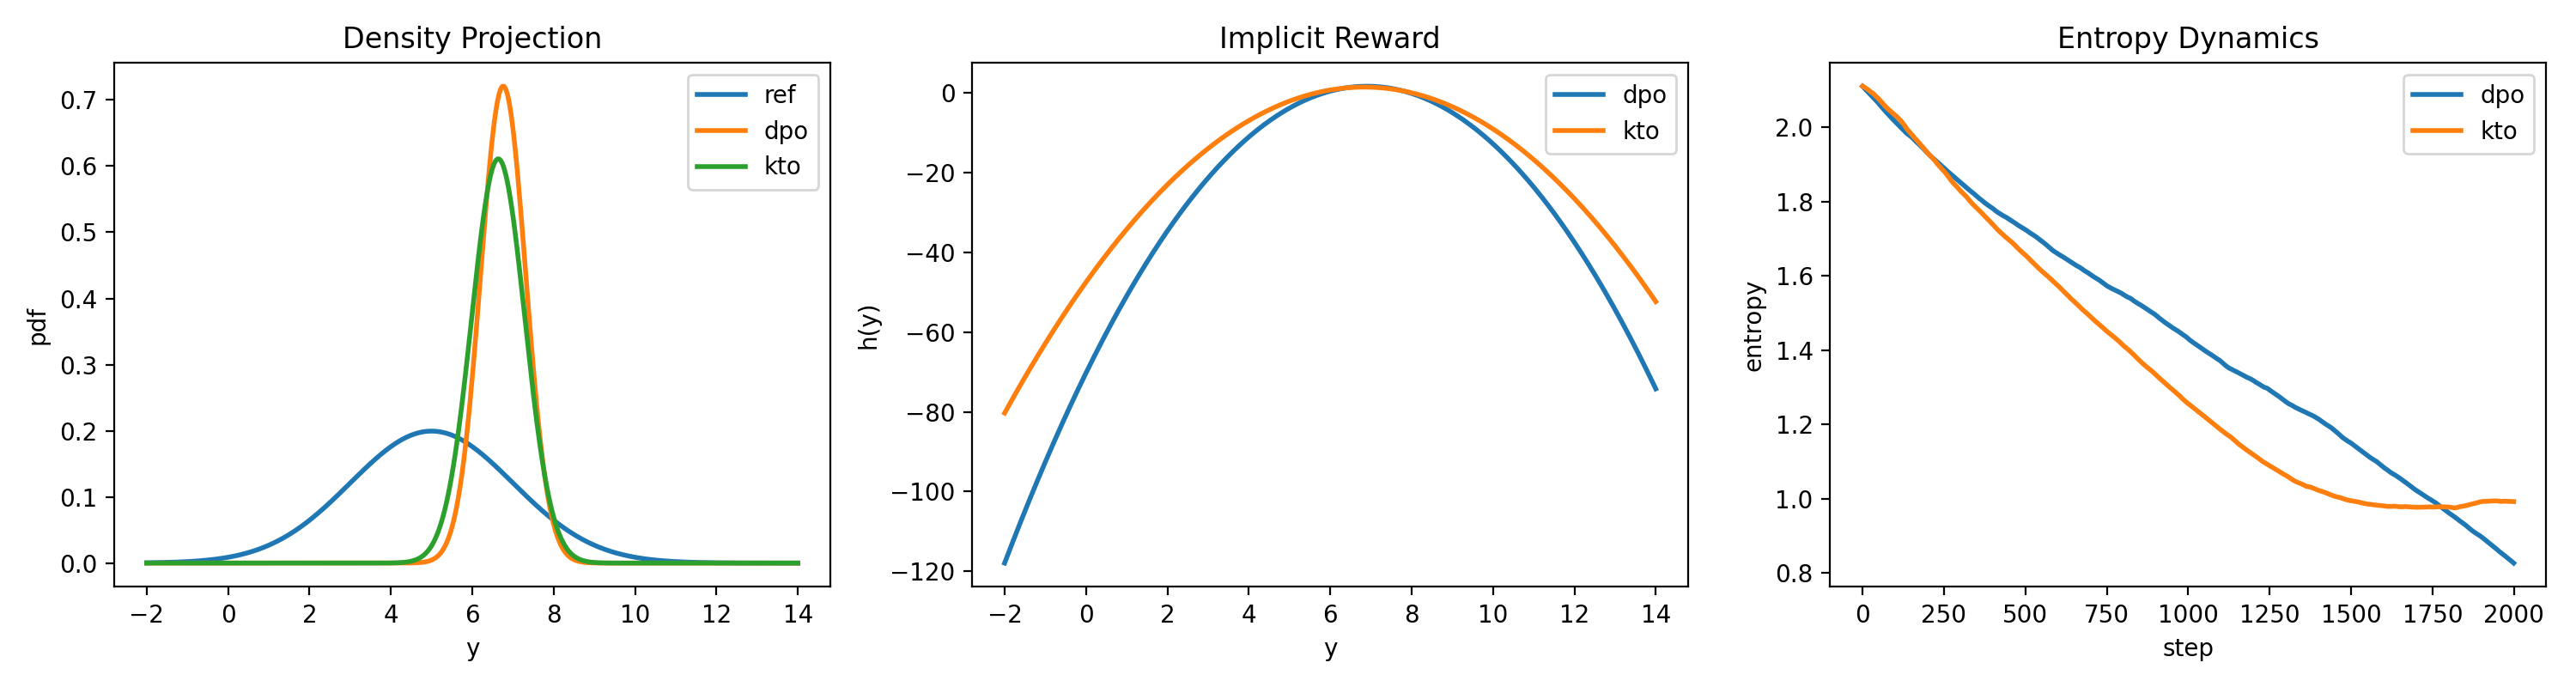
\includegraphics[width=0.95\textwidth]{figures/single_main_panels.png}
    \caption{Main panels: density projection, implicit reward, and entropy dynamics.}
\end{figure}

\subsection{Quartile Evolution (0/25/50/75/100\%)}
\begin{figure}[H]
    \centering
    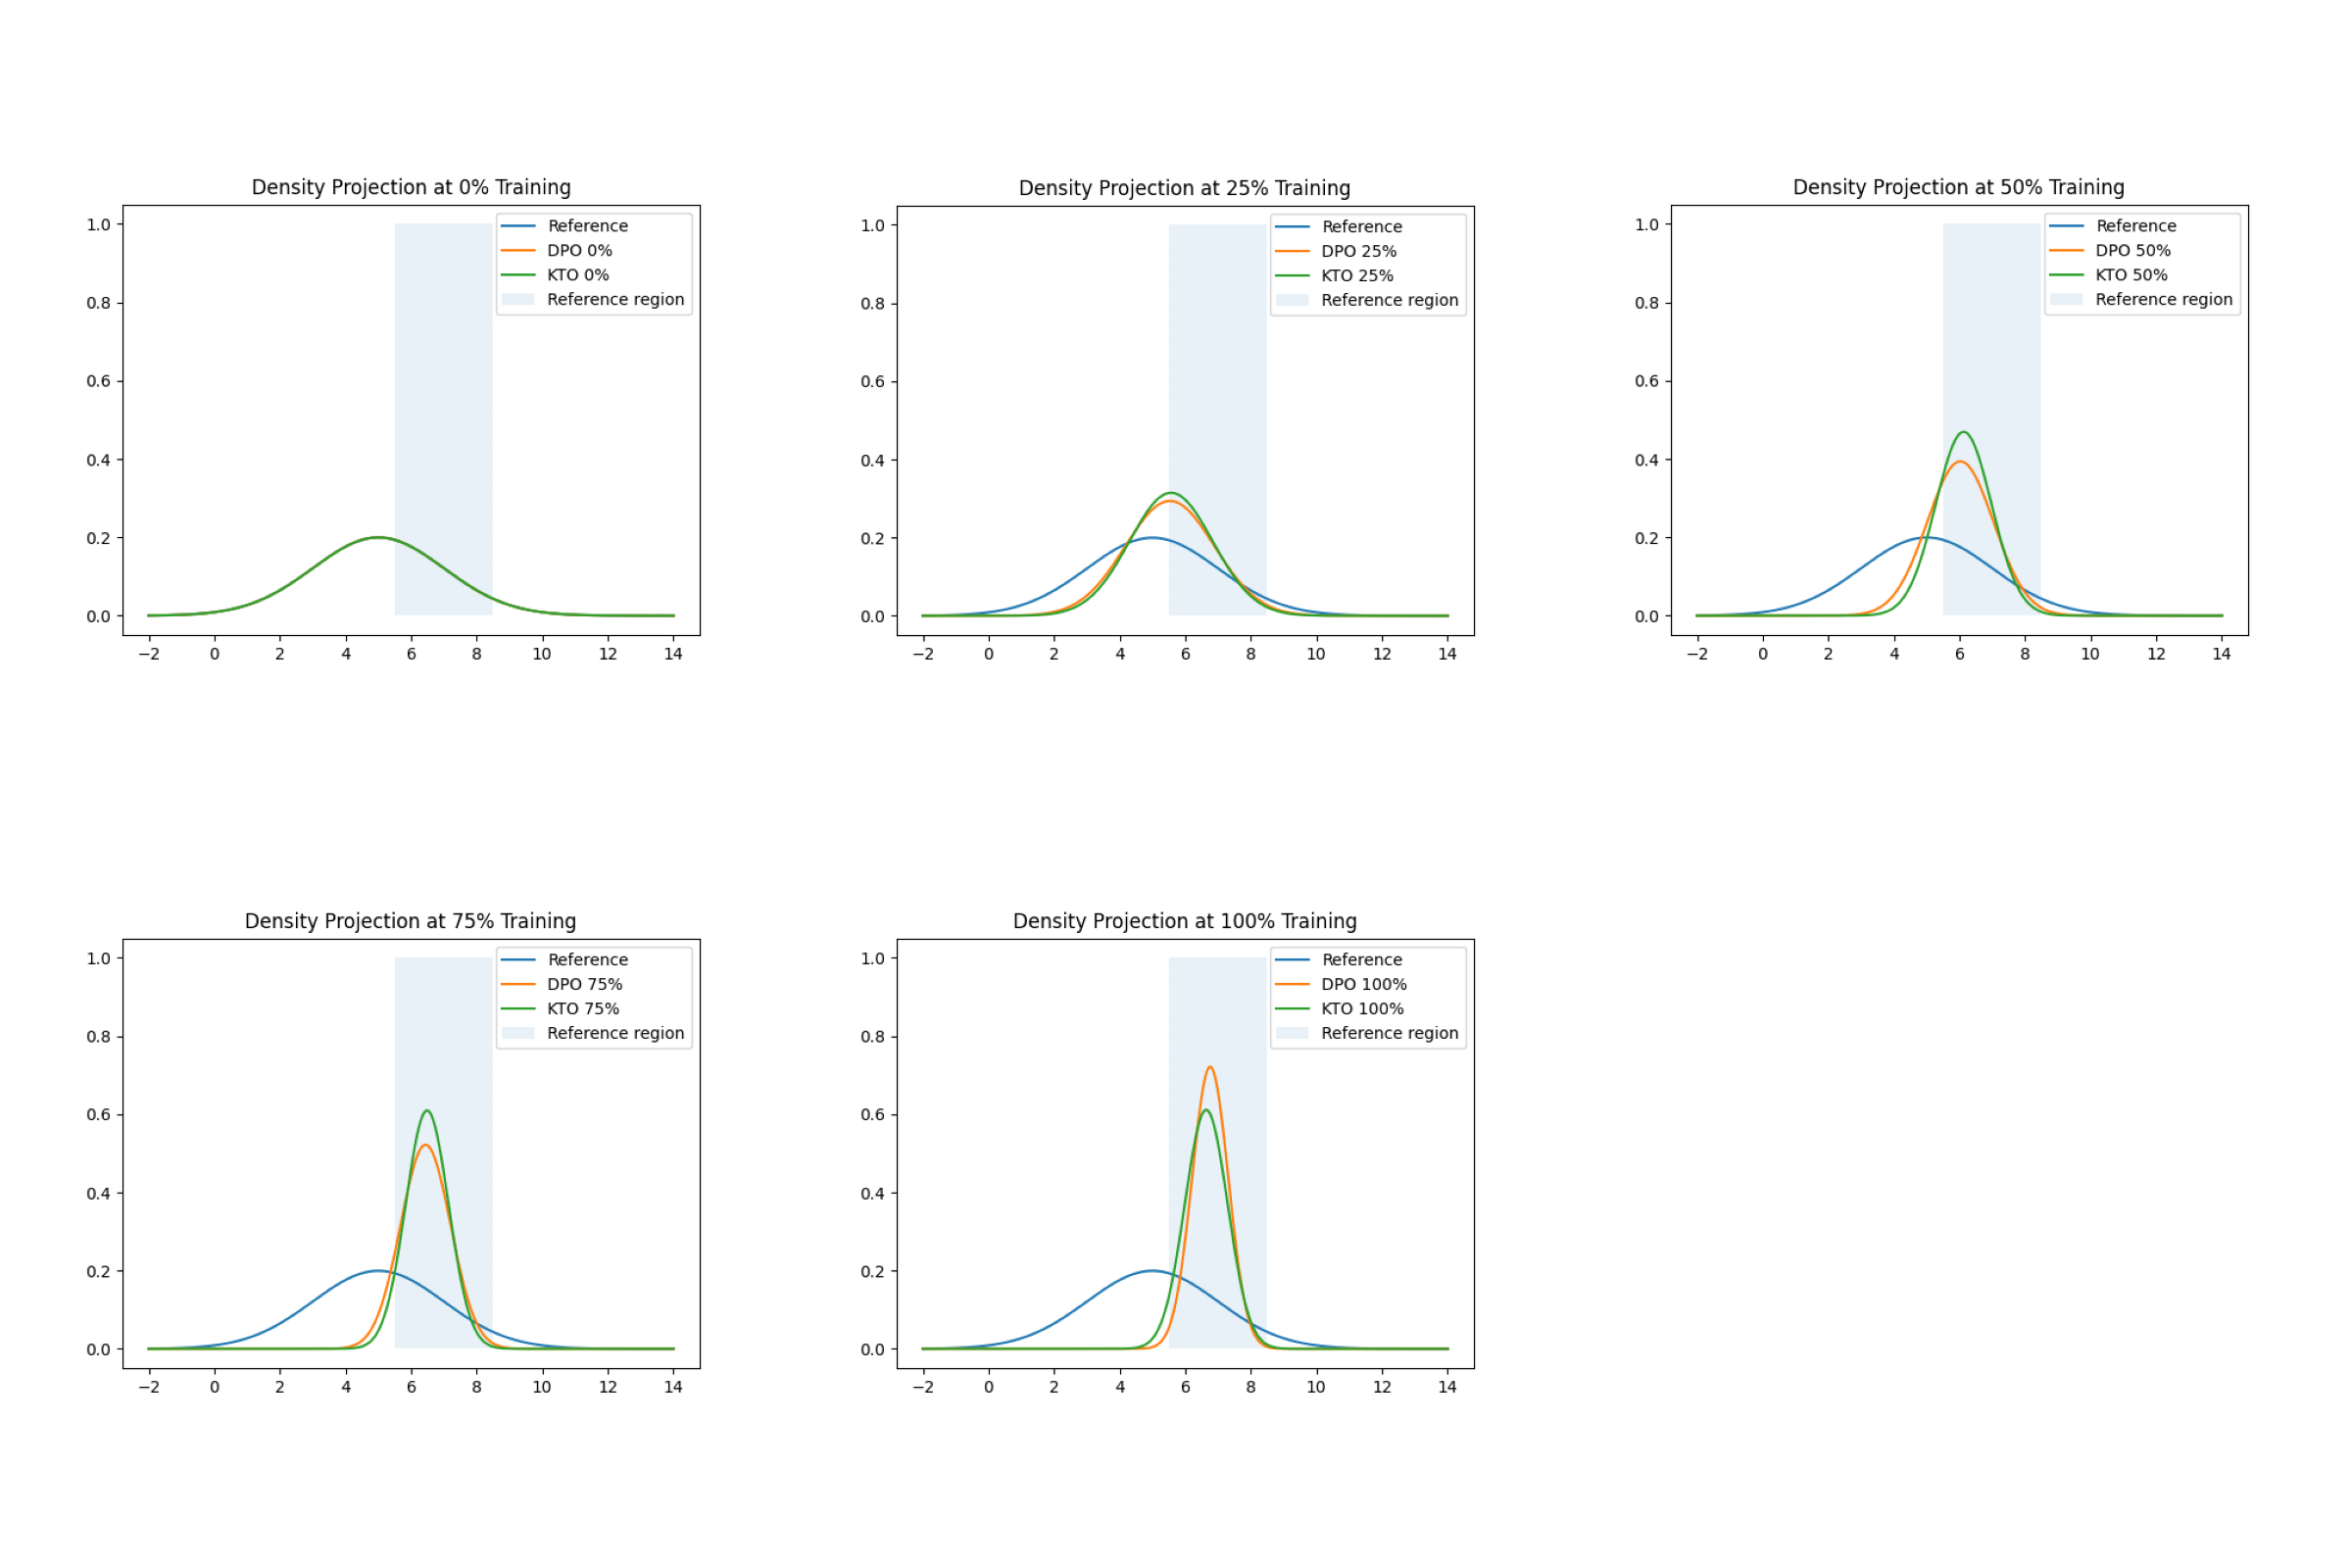
\includegraphics[width=0.95\textwidth]{figures/single_density_montage.png}
    \caption{Density evolution montage (quartiles).}
\end{figure}

\subsection{KL Estimation Modes (Reference Sampling)}
\begin{figure}[H]
    \centering
    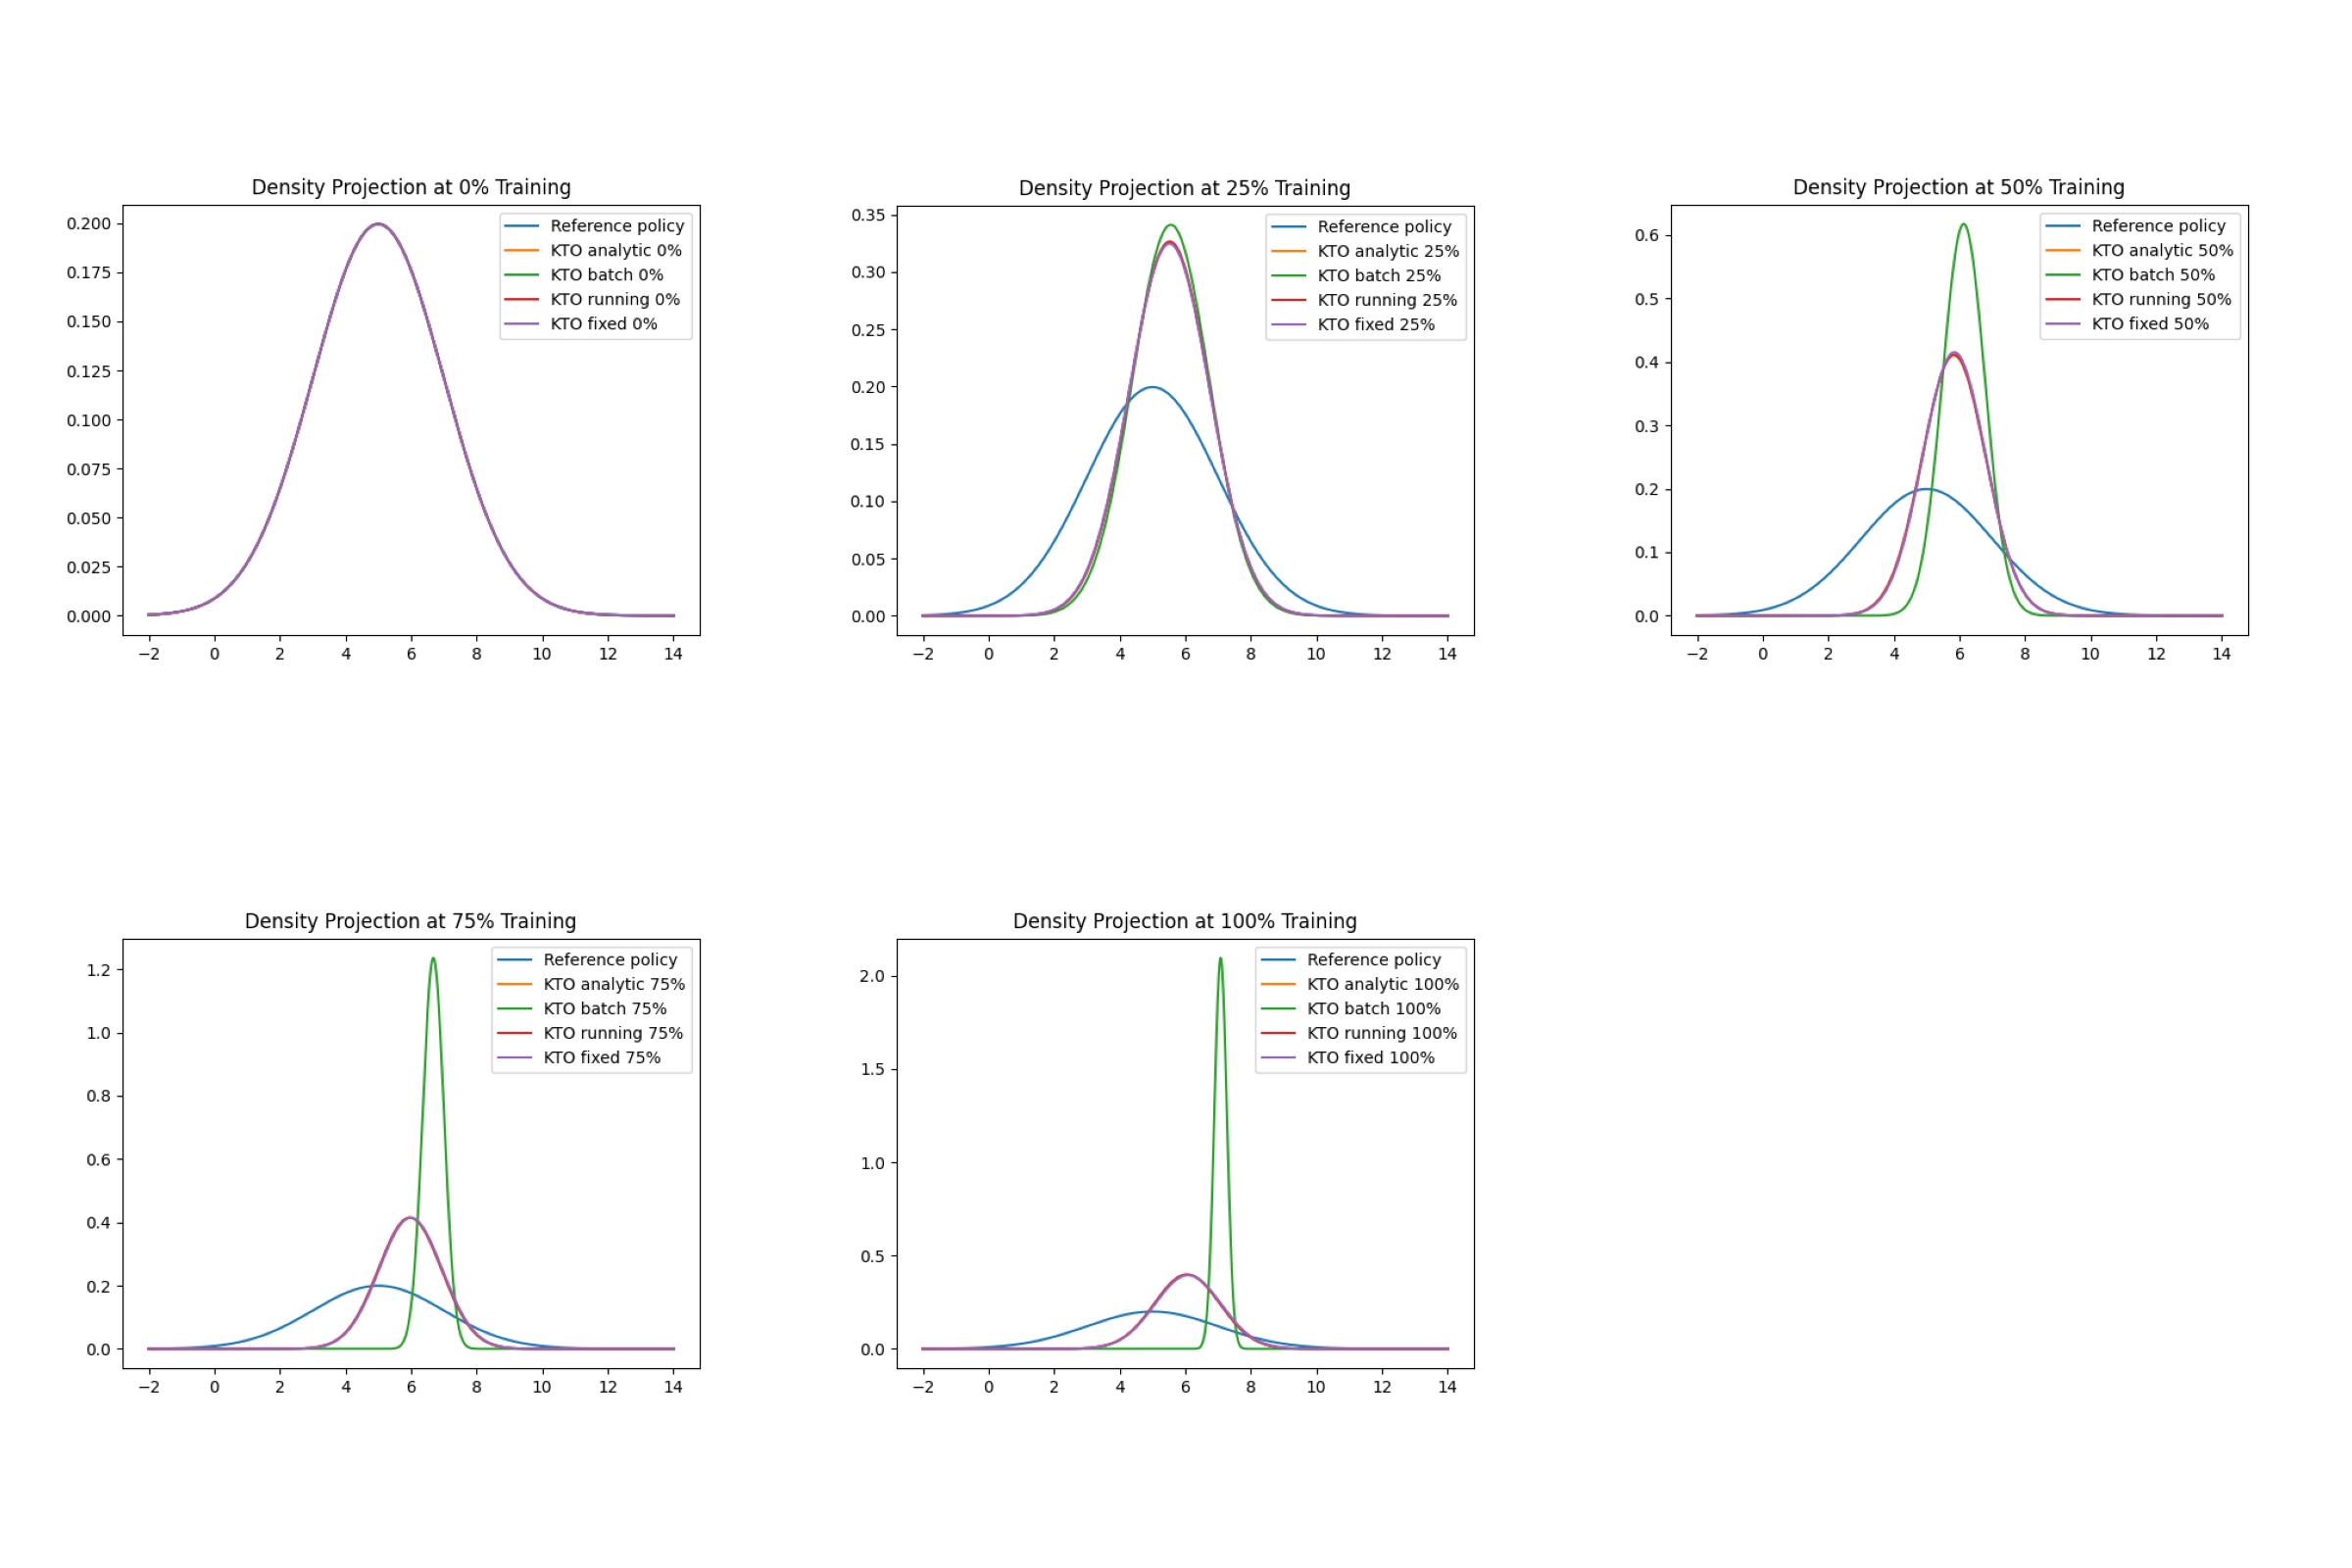
\includegraphics[width=0.95\textwidth]{figures/single_reference_sampling_montage.png}
    \caption{KTO density at quartiles for different KL estimation modes.}
\end{figure}

\subsection{Sensitivity Tests}
\begin{figure}[H]
    \centering
    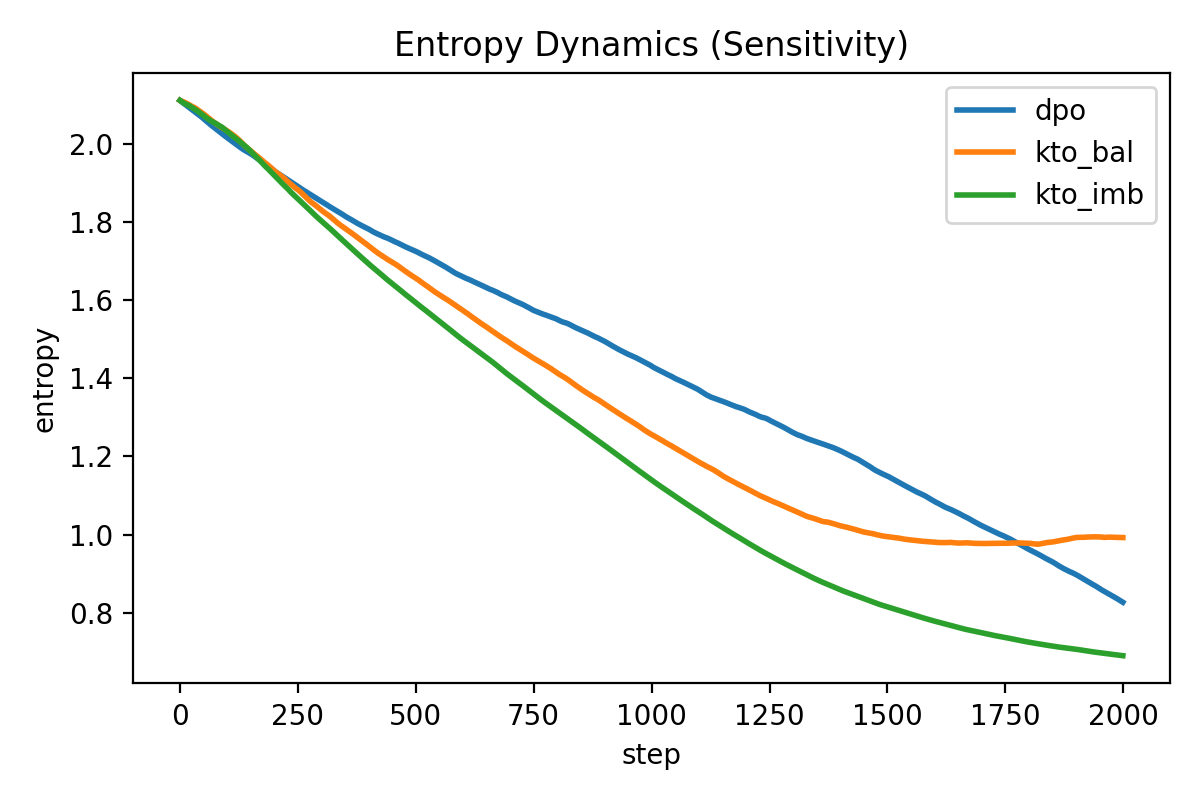
\includegraphics[width=0.85\textwidth]{figures/single_entropy_sensitivity.png}
    \caption{Balanced vs. imbalanced KTO entropy dynamics.}
\end{figure}

\begin{figure}[H]
    \centering
    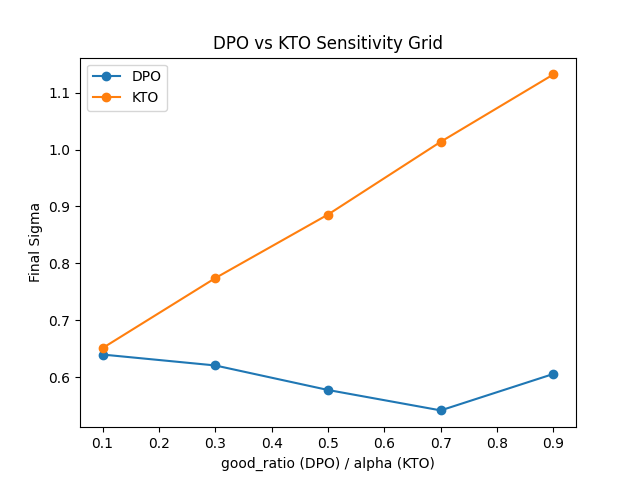
\includegraphics[width=0.85\textwidth]{figures/single_data_sensitivity.png}
    \caption{Sensitivity grid: final sigma vs. DPO good\_ratio and KTO supervision ratio.}
\end{figure}

\subsection{Beta and Zone Width Sweeps}
\begin{figure}[H]
    \centering
    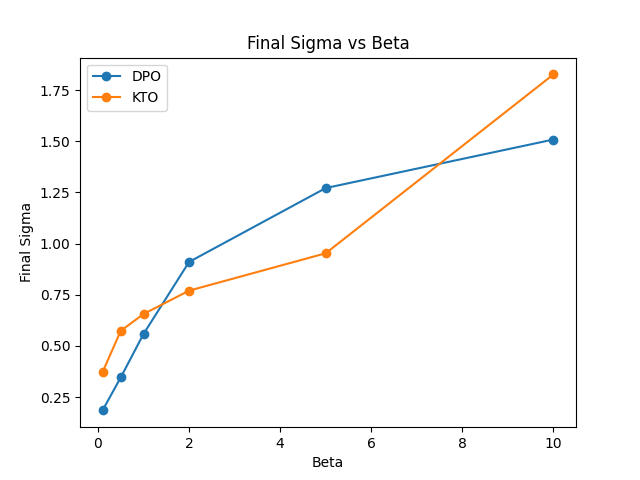
\includegraphics[width=0.8\textwidth]{figures/single_beta_sweep.png}
    \caption{Final sigma vs. $\beta$.}
\end{figure}

\begin{figure}[H]
    \centering
    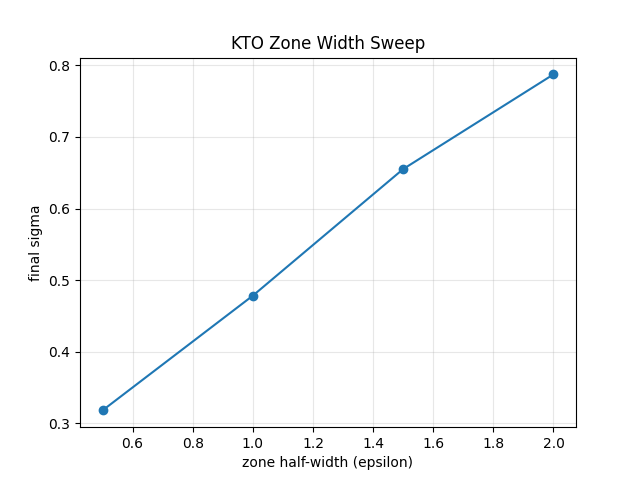
\includegraphics[width=0.8\textwidth]{figures/single_kto_zone_sweep.png}
    \caption{KTO final sigma vs. zone half-width.}
\end{figure}

\section{Initialization Sensitivity (Single Gaussian)}
\begin{figure}[H]
    \centering
    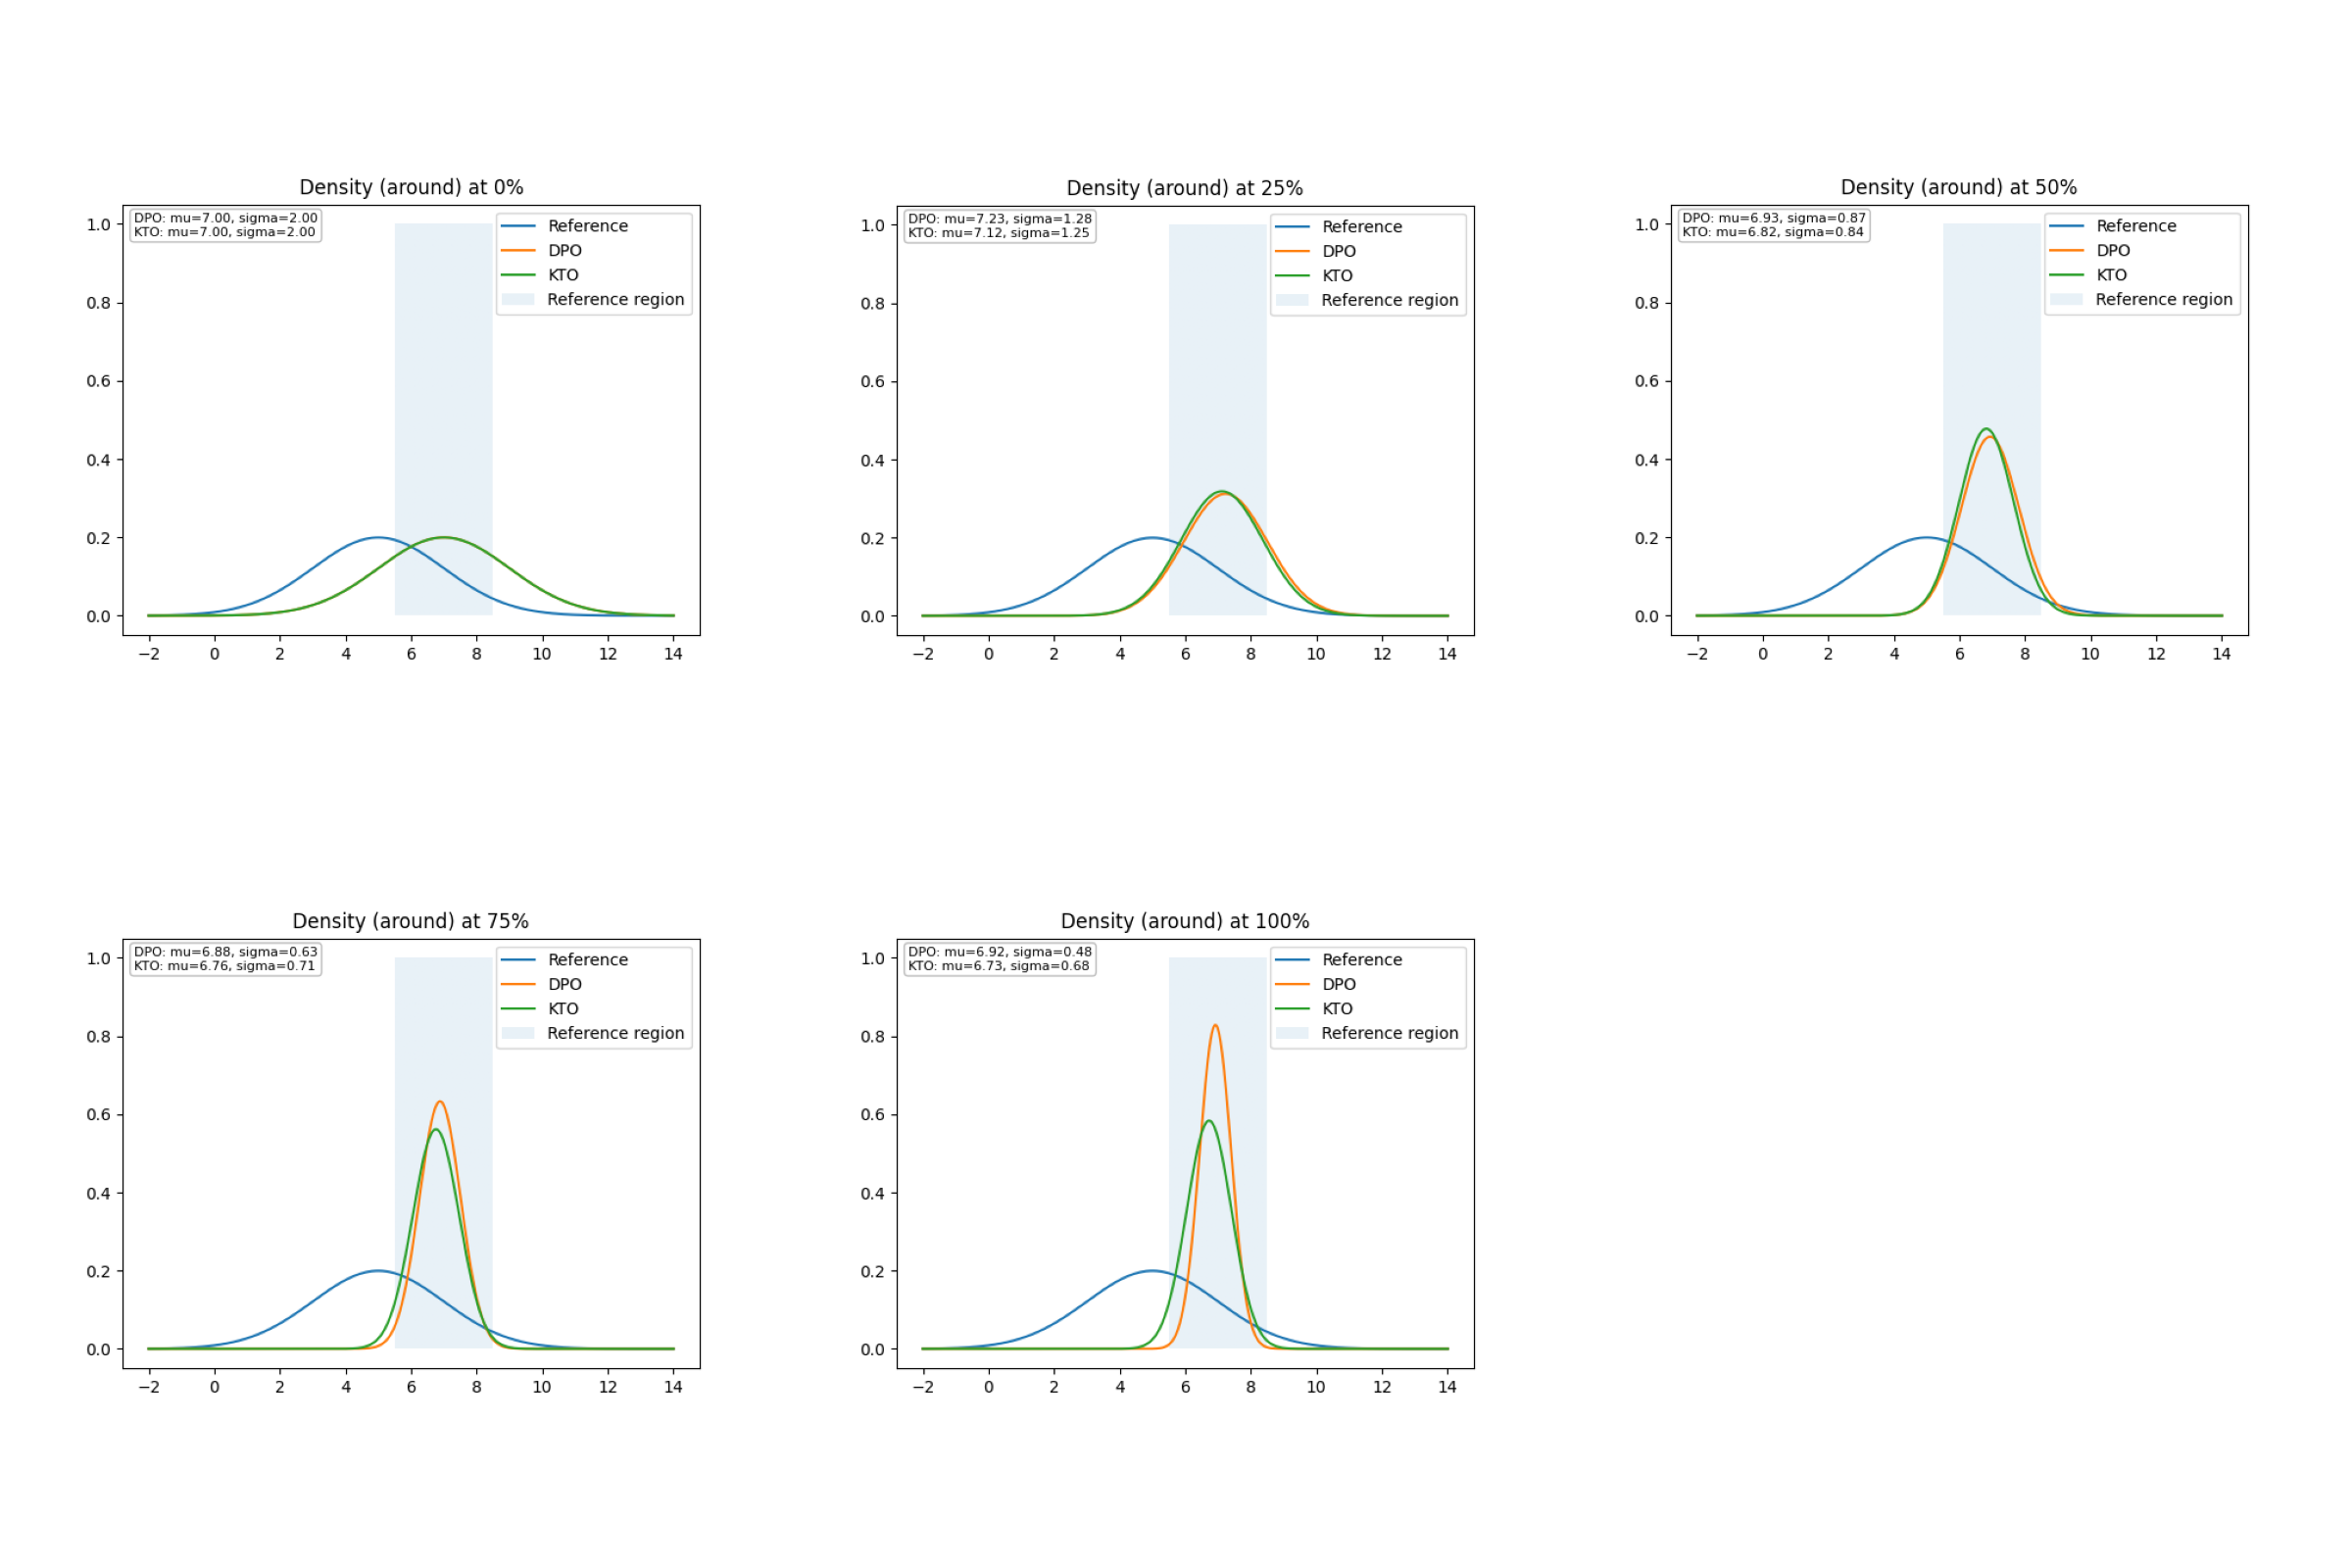
\includegraphics[width=0.95\textwidth]{figures/single_init_density_around.png}
    \caption{Init around 7: density evolution montage.}
\end{figure}

\begin{figure}[H]
    \centering
    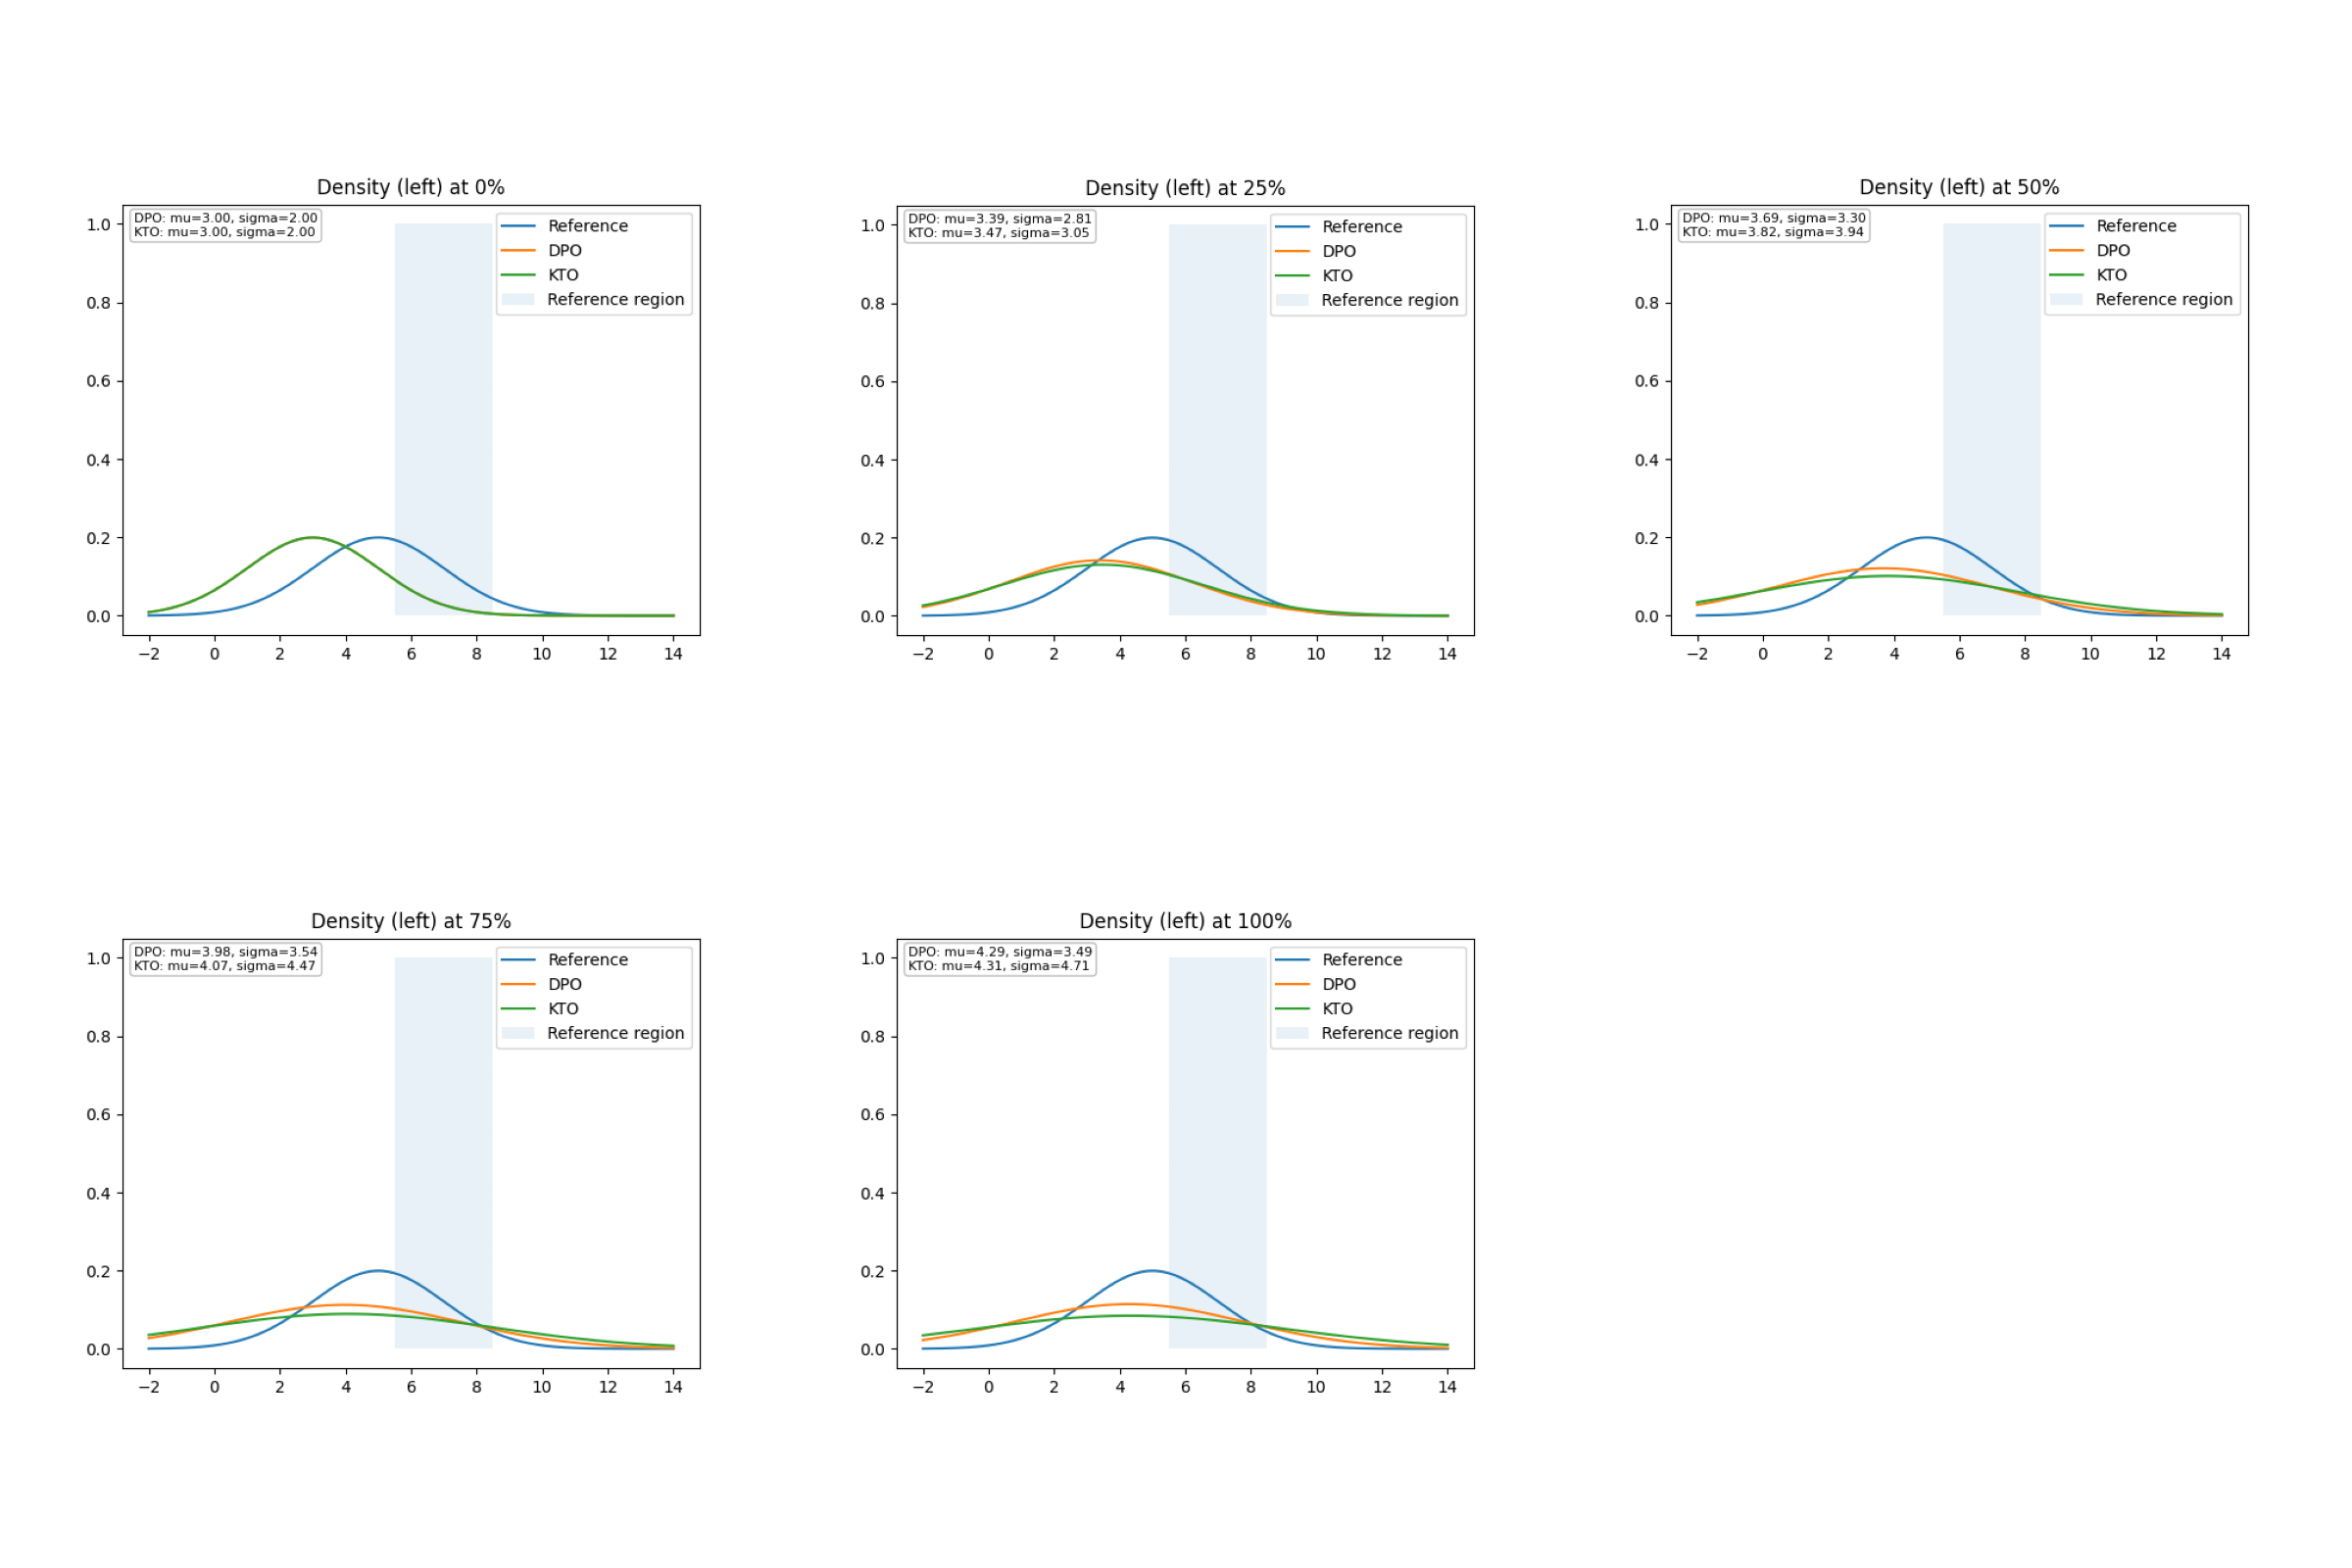
\includegraphics[width=0.95\textwidth]{figures/single_init_density_left.png}
    \caption{Init left of 7: density evolution montage.}
\end{figure}

\begin{figure}[H]
    \centering
    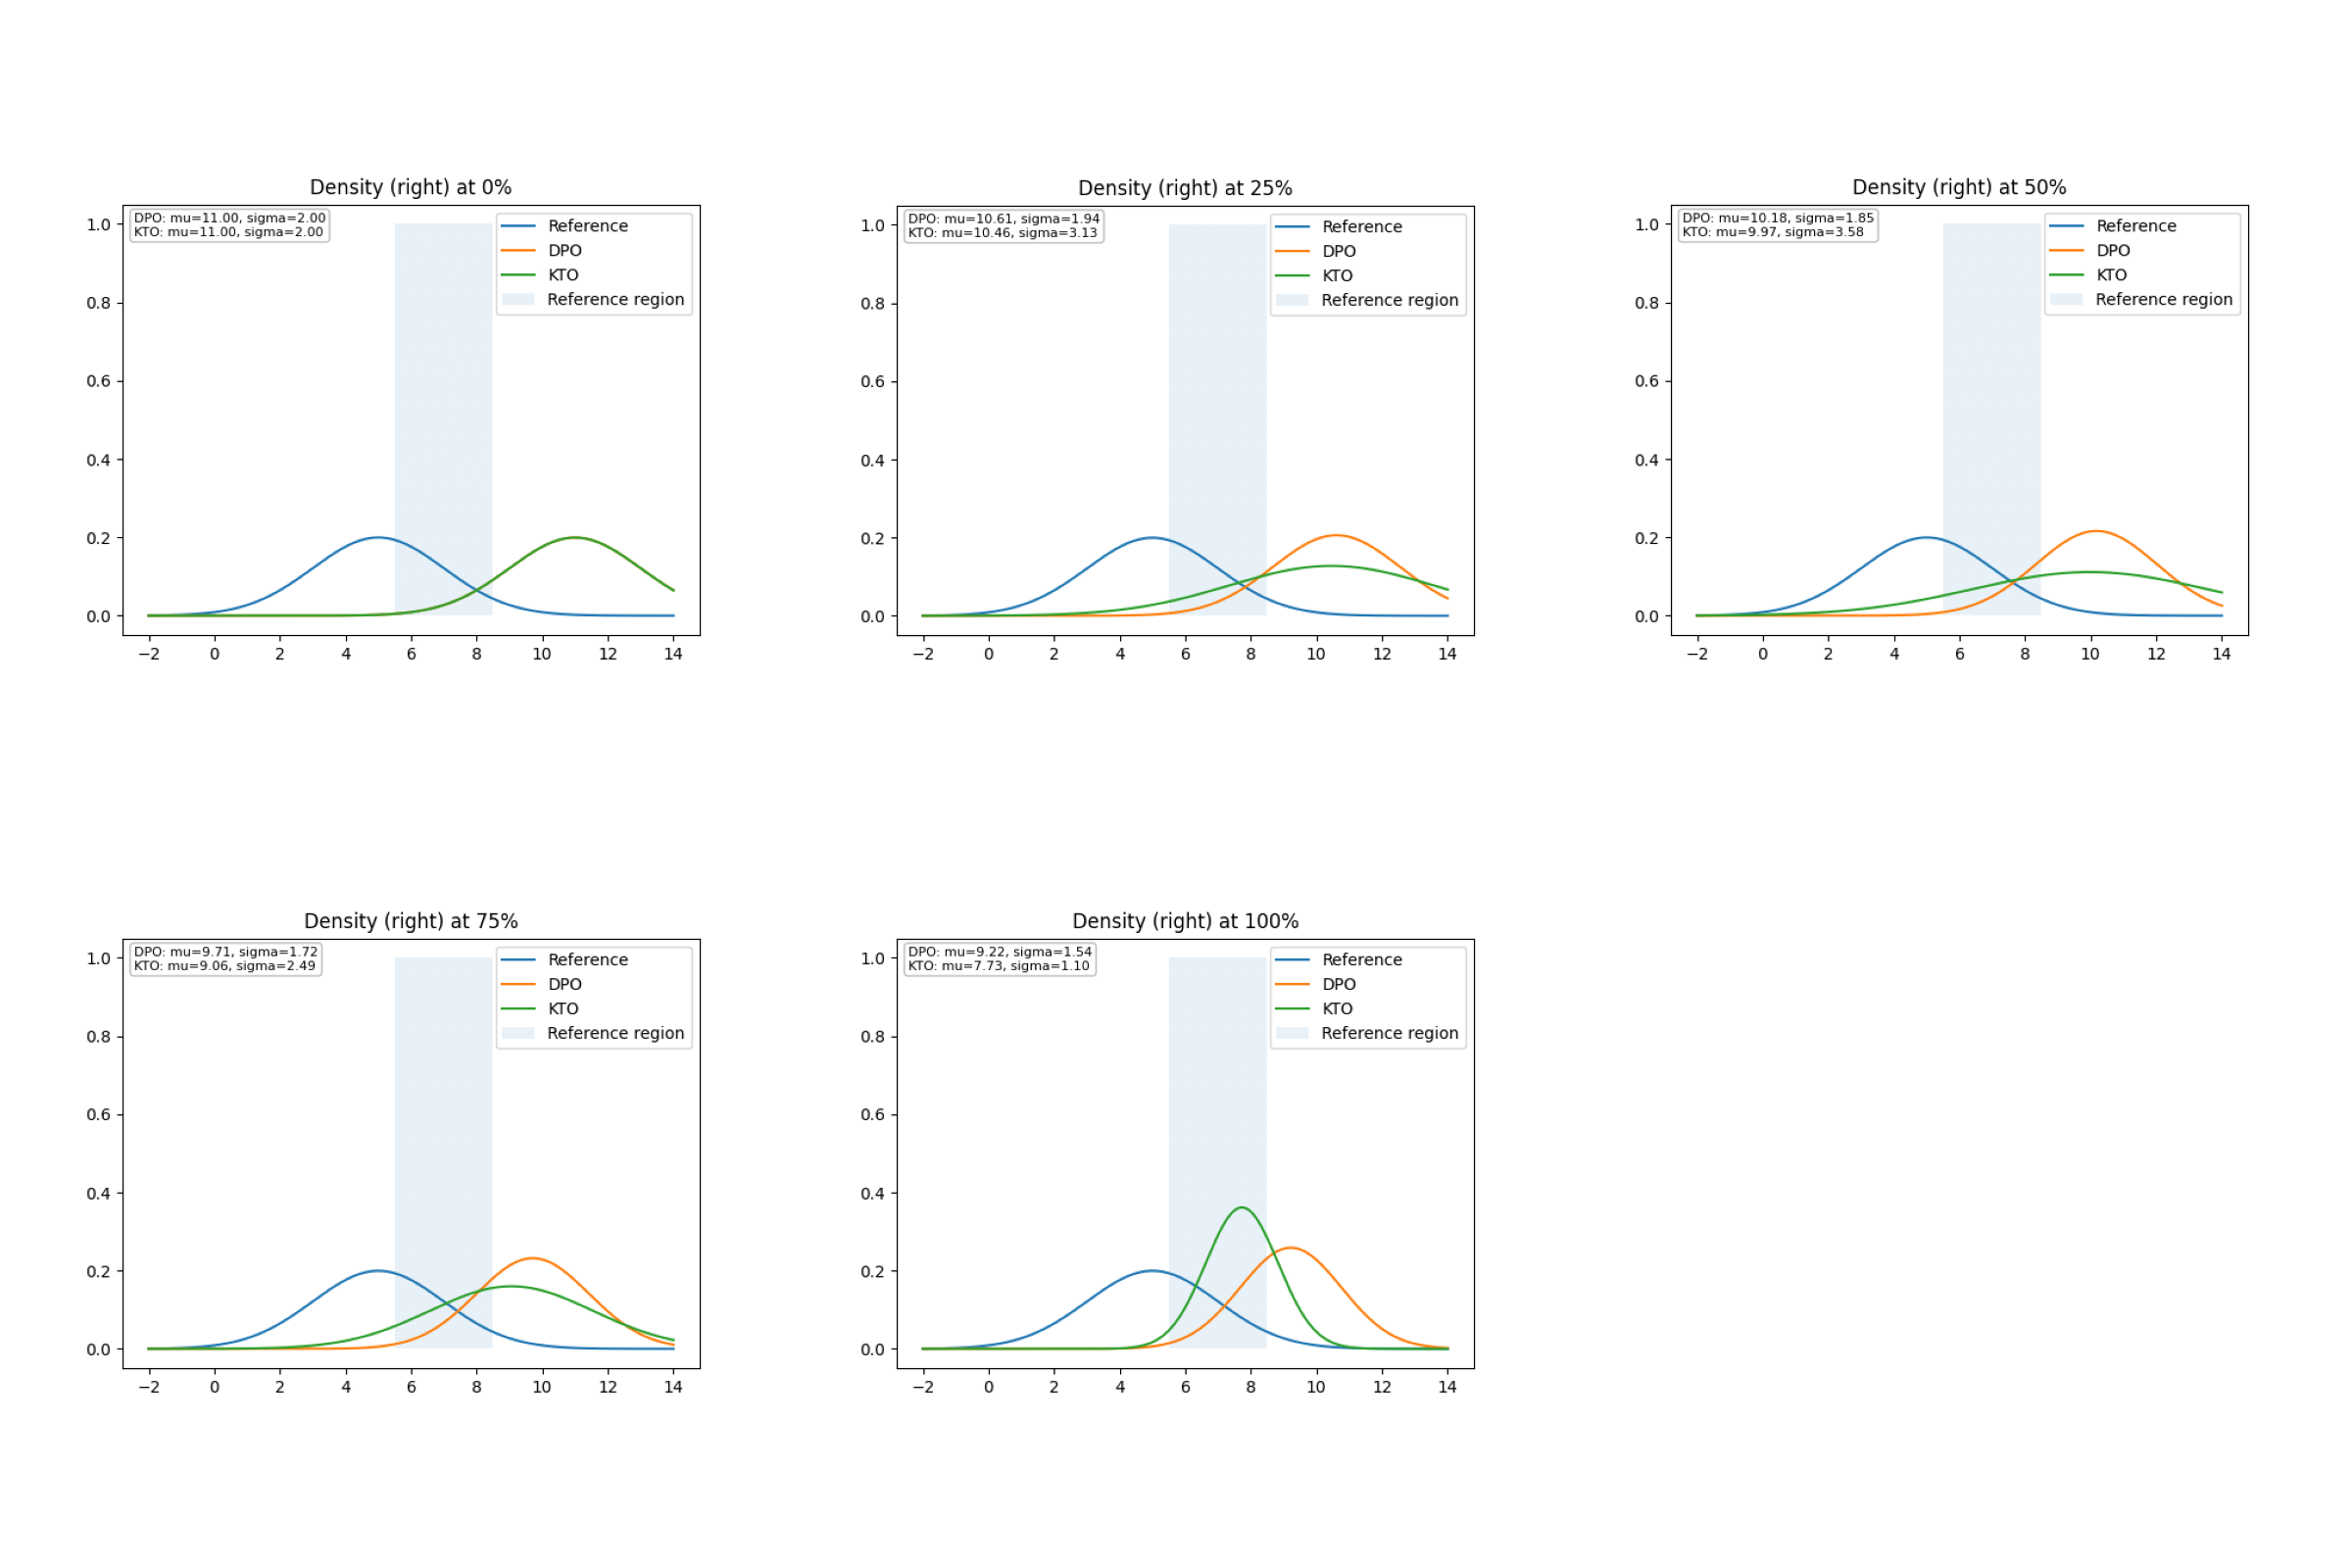
\includegraphics[width=0.95\textwidth]{figures/single_init_density_right.png}
    \caption{Init right of 7: density evolution montage.}
\end{figure}

\section{Mixture Extensions}
\subsection{Mixture Density and Final Implicit Reward}
\begin{figure}[H]
    \centering
    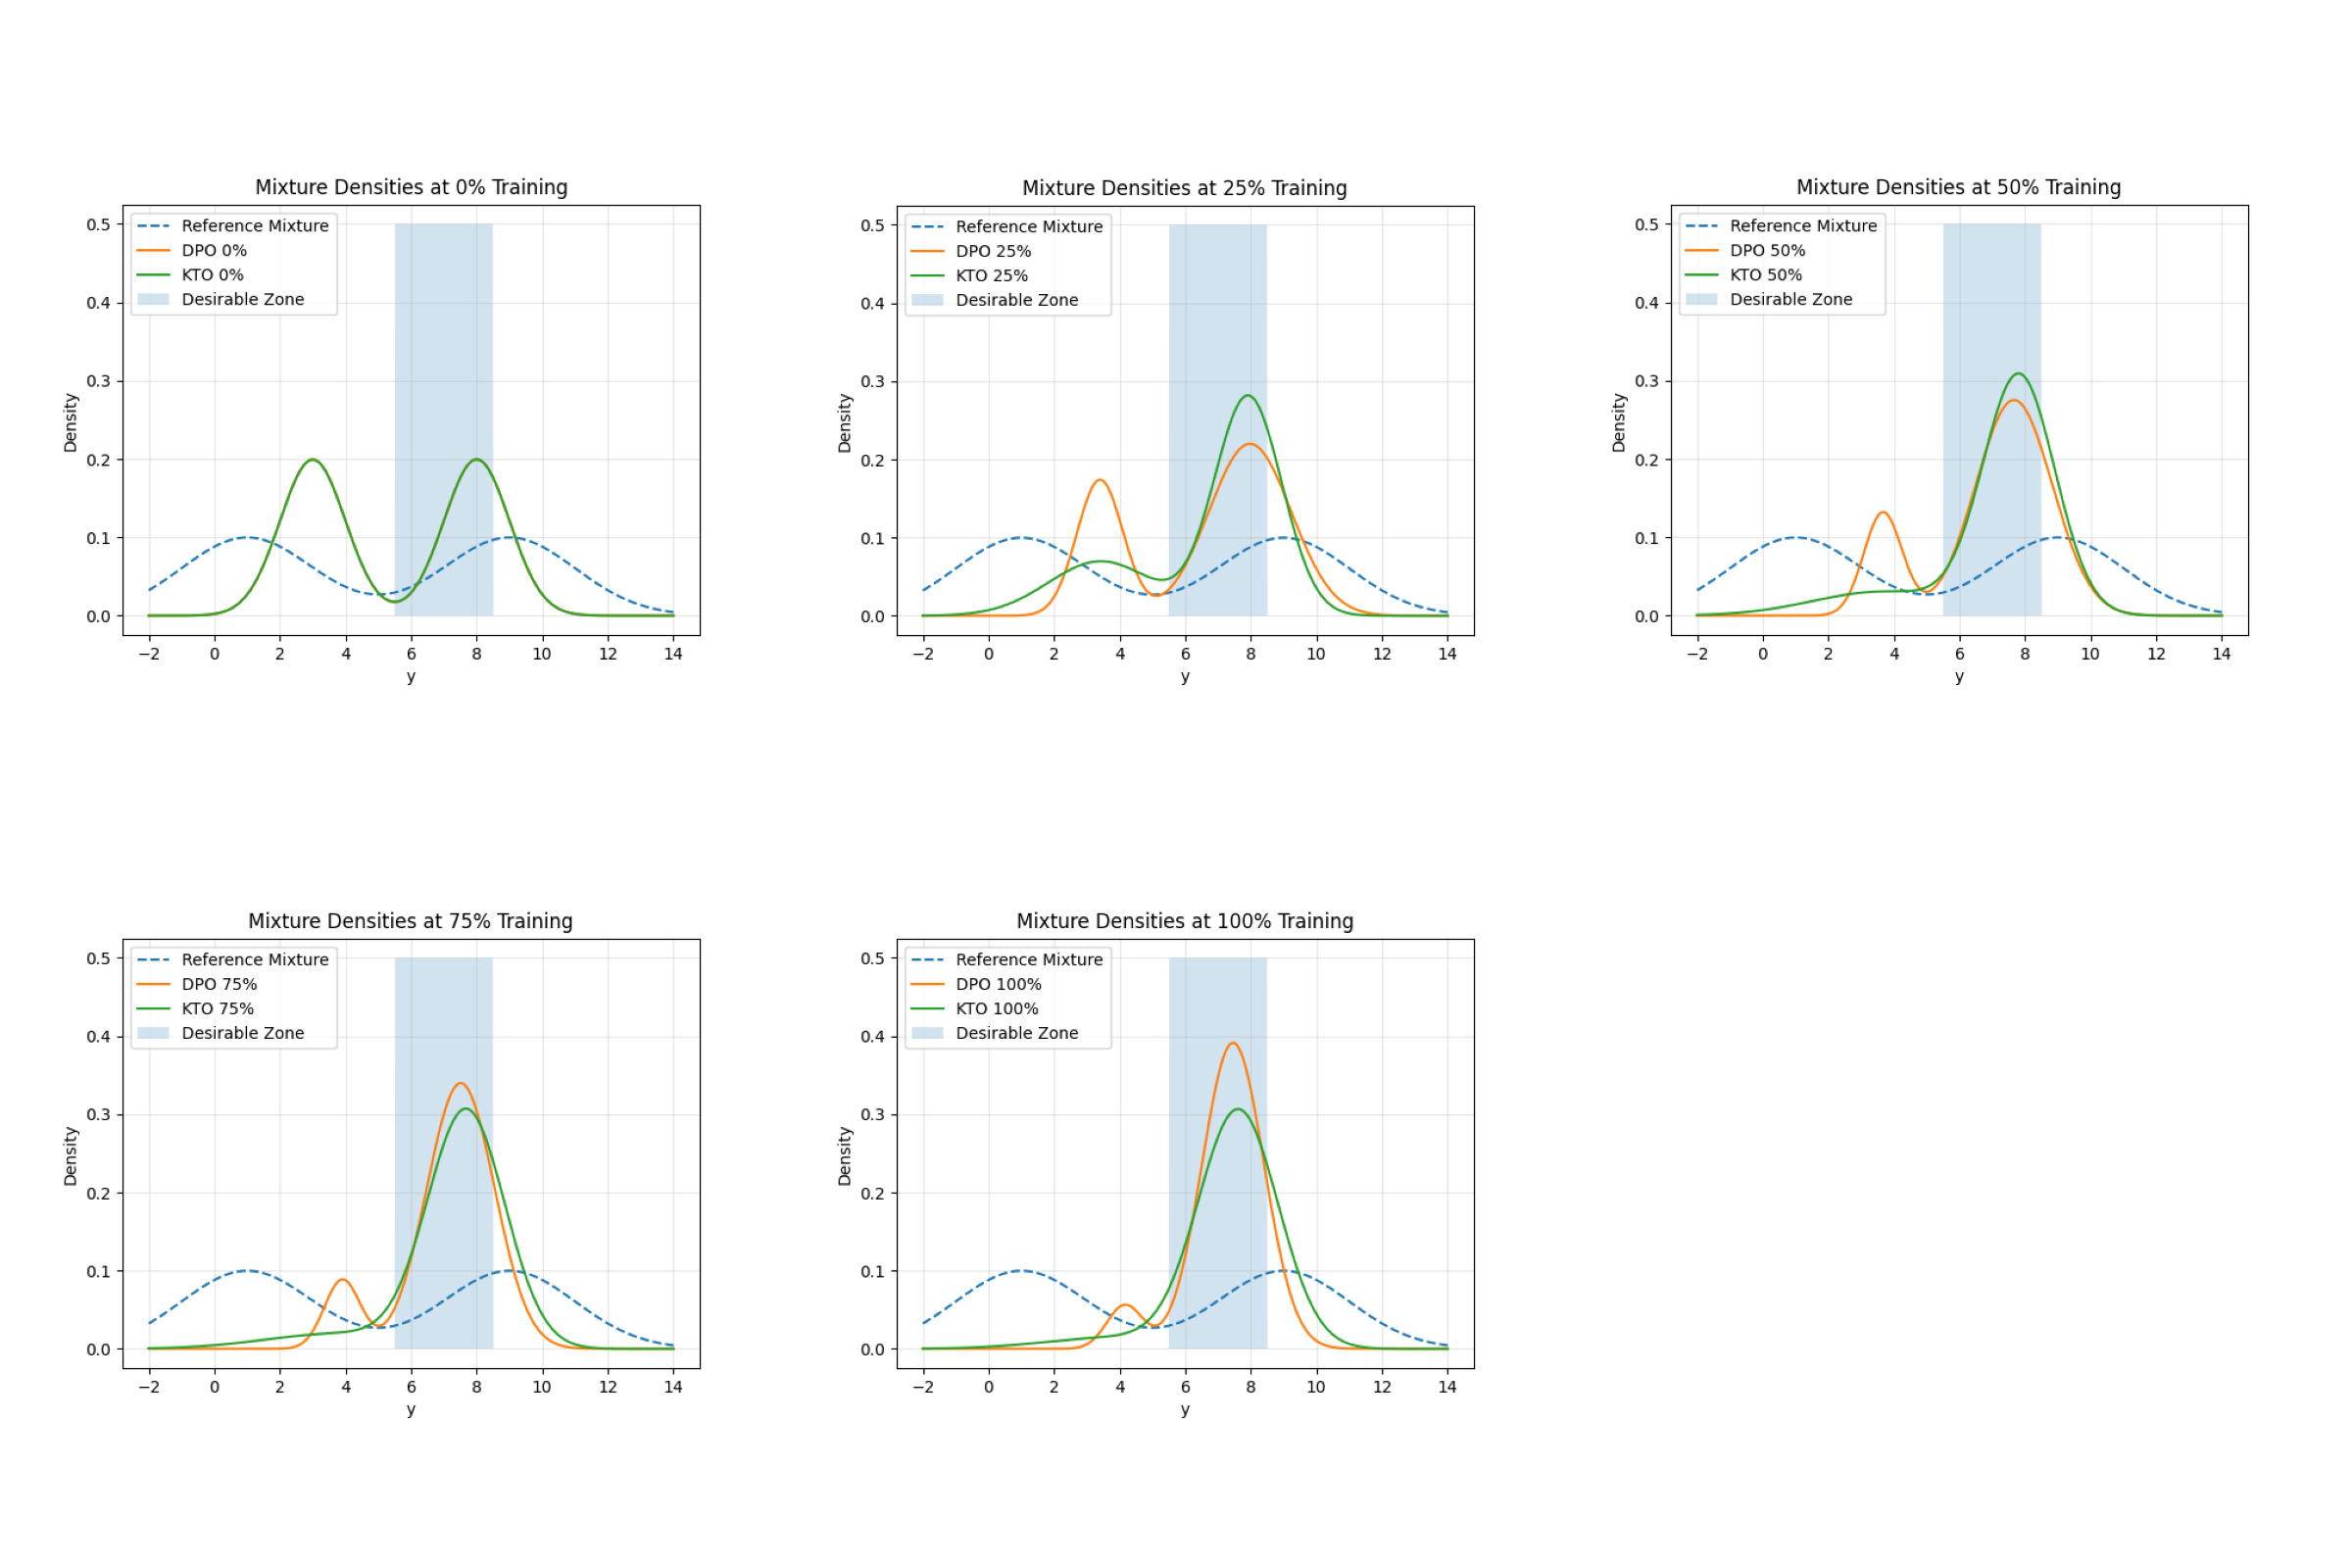
\includegraphics[width=0.95\textwidth]{figures/mix_density_montage.png}
    \caption{Mixture density evolution montage.}
\end{figure}

\subsection{KL Modes in Mixtures}
\begin{figure}[H]
    \centering
    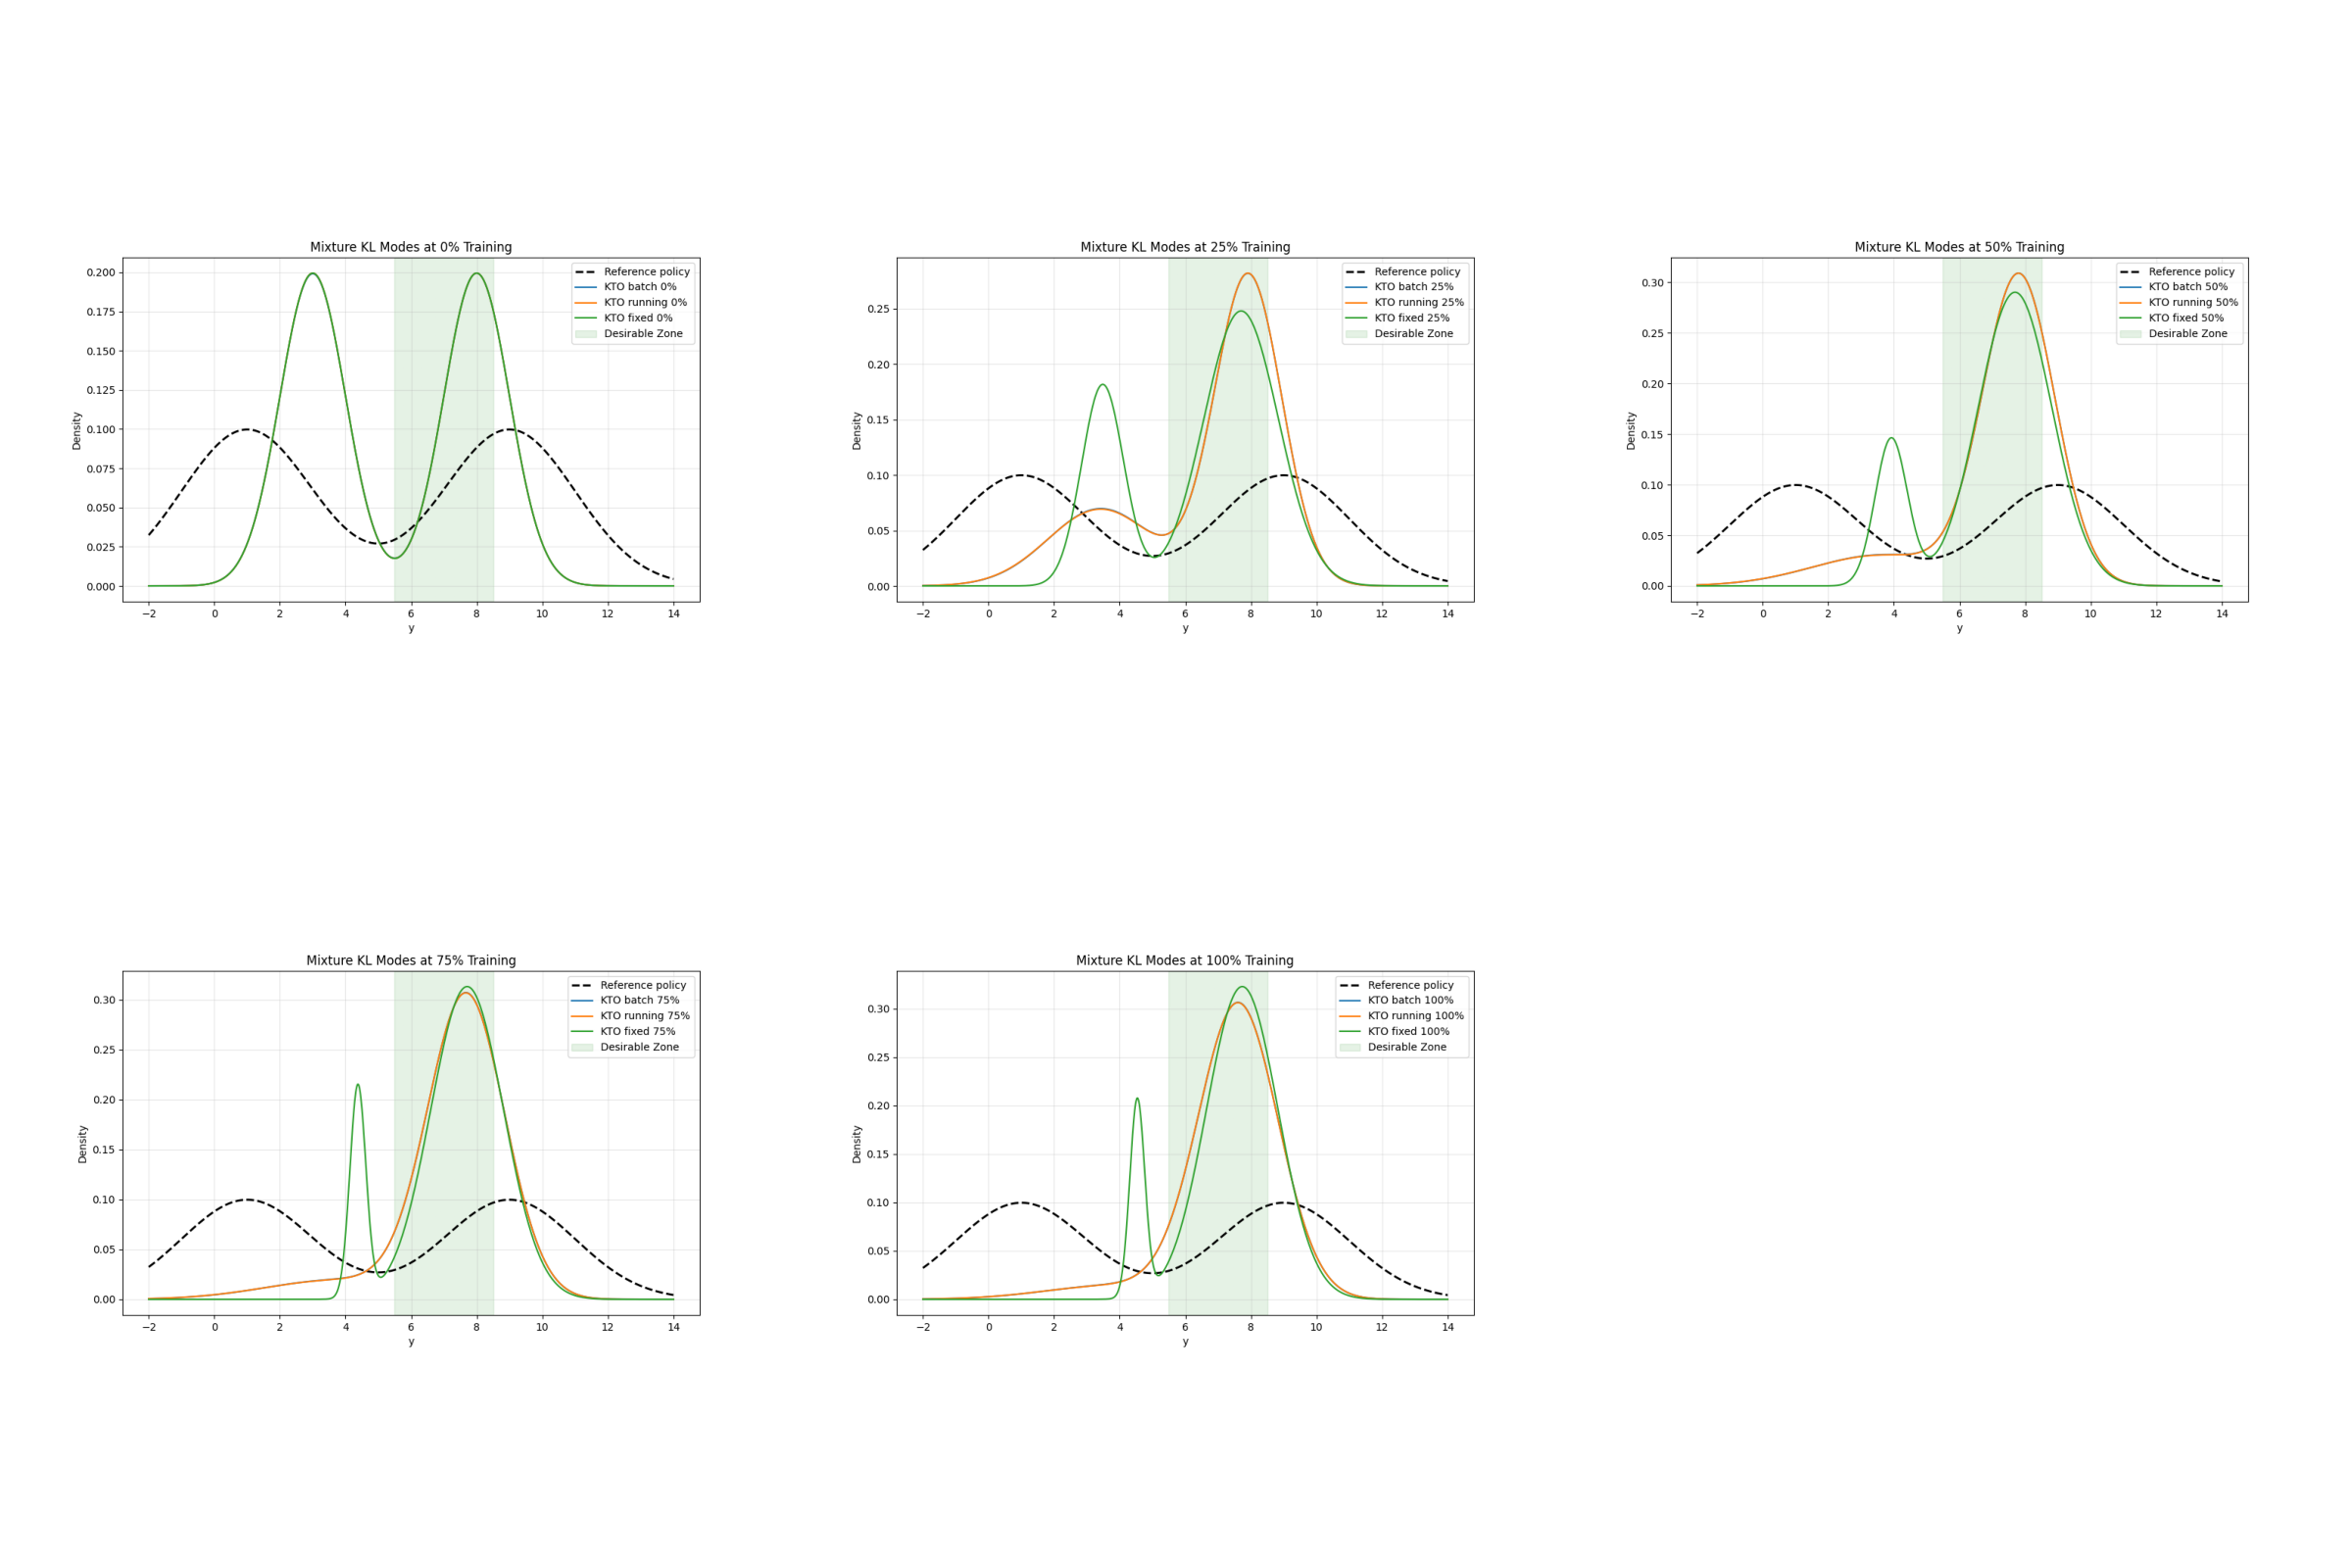
\includegraphics[width=0.95\textwidth]{figures/mix_reference_sampling_montage.png}
    \caption{Mixture KTO densities across KL modes (quartiles).}
\end{figure}

\begin{figure}[H]
    \centering
    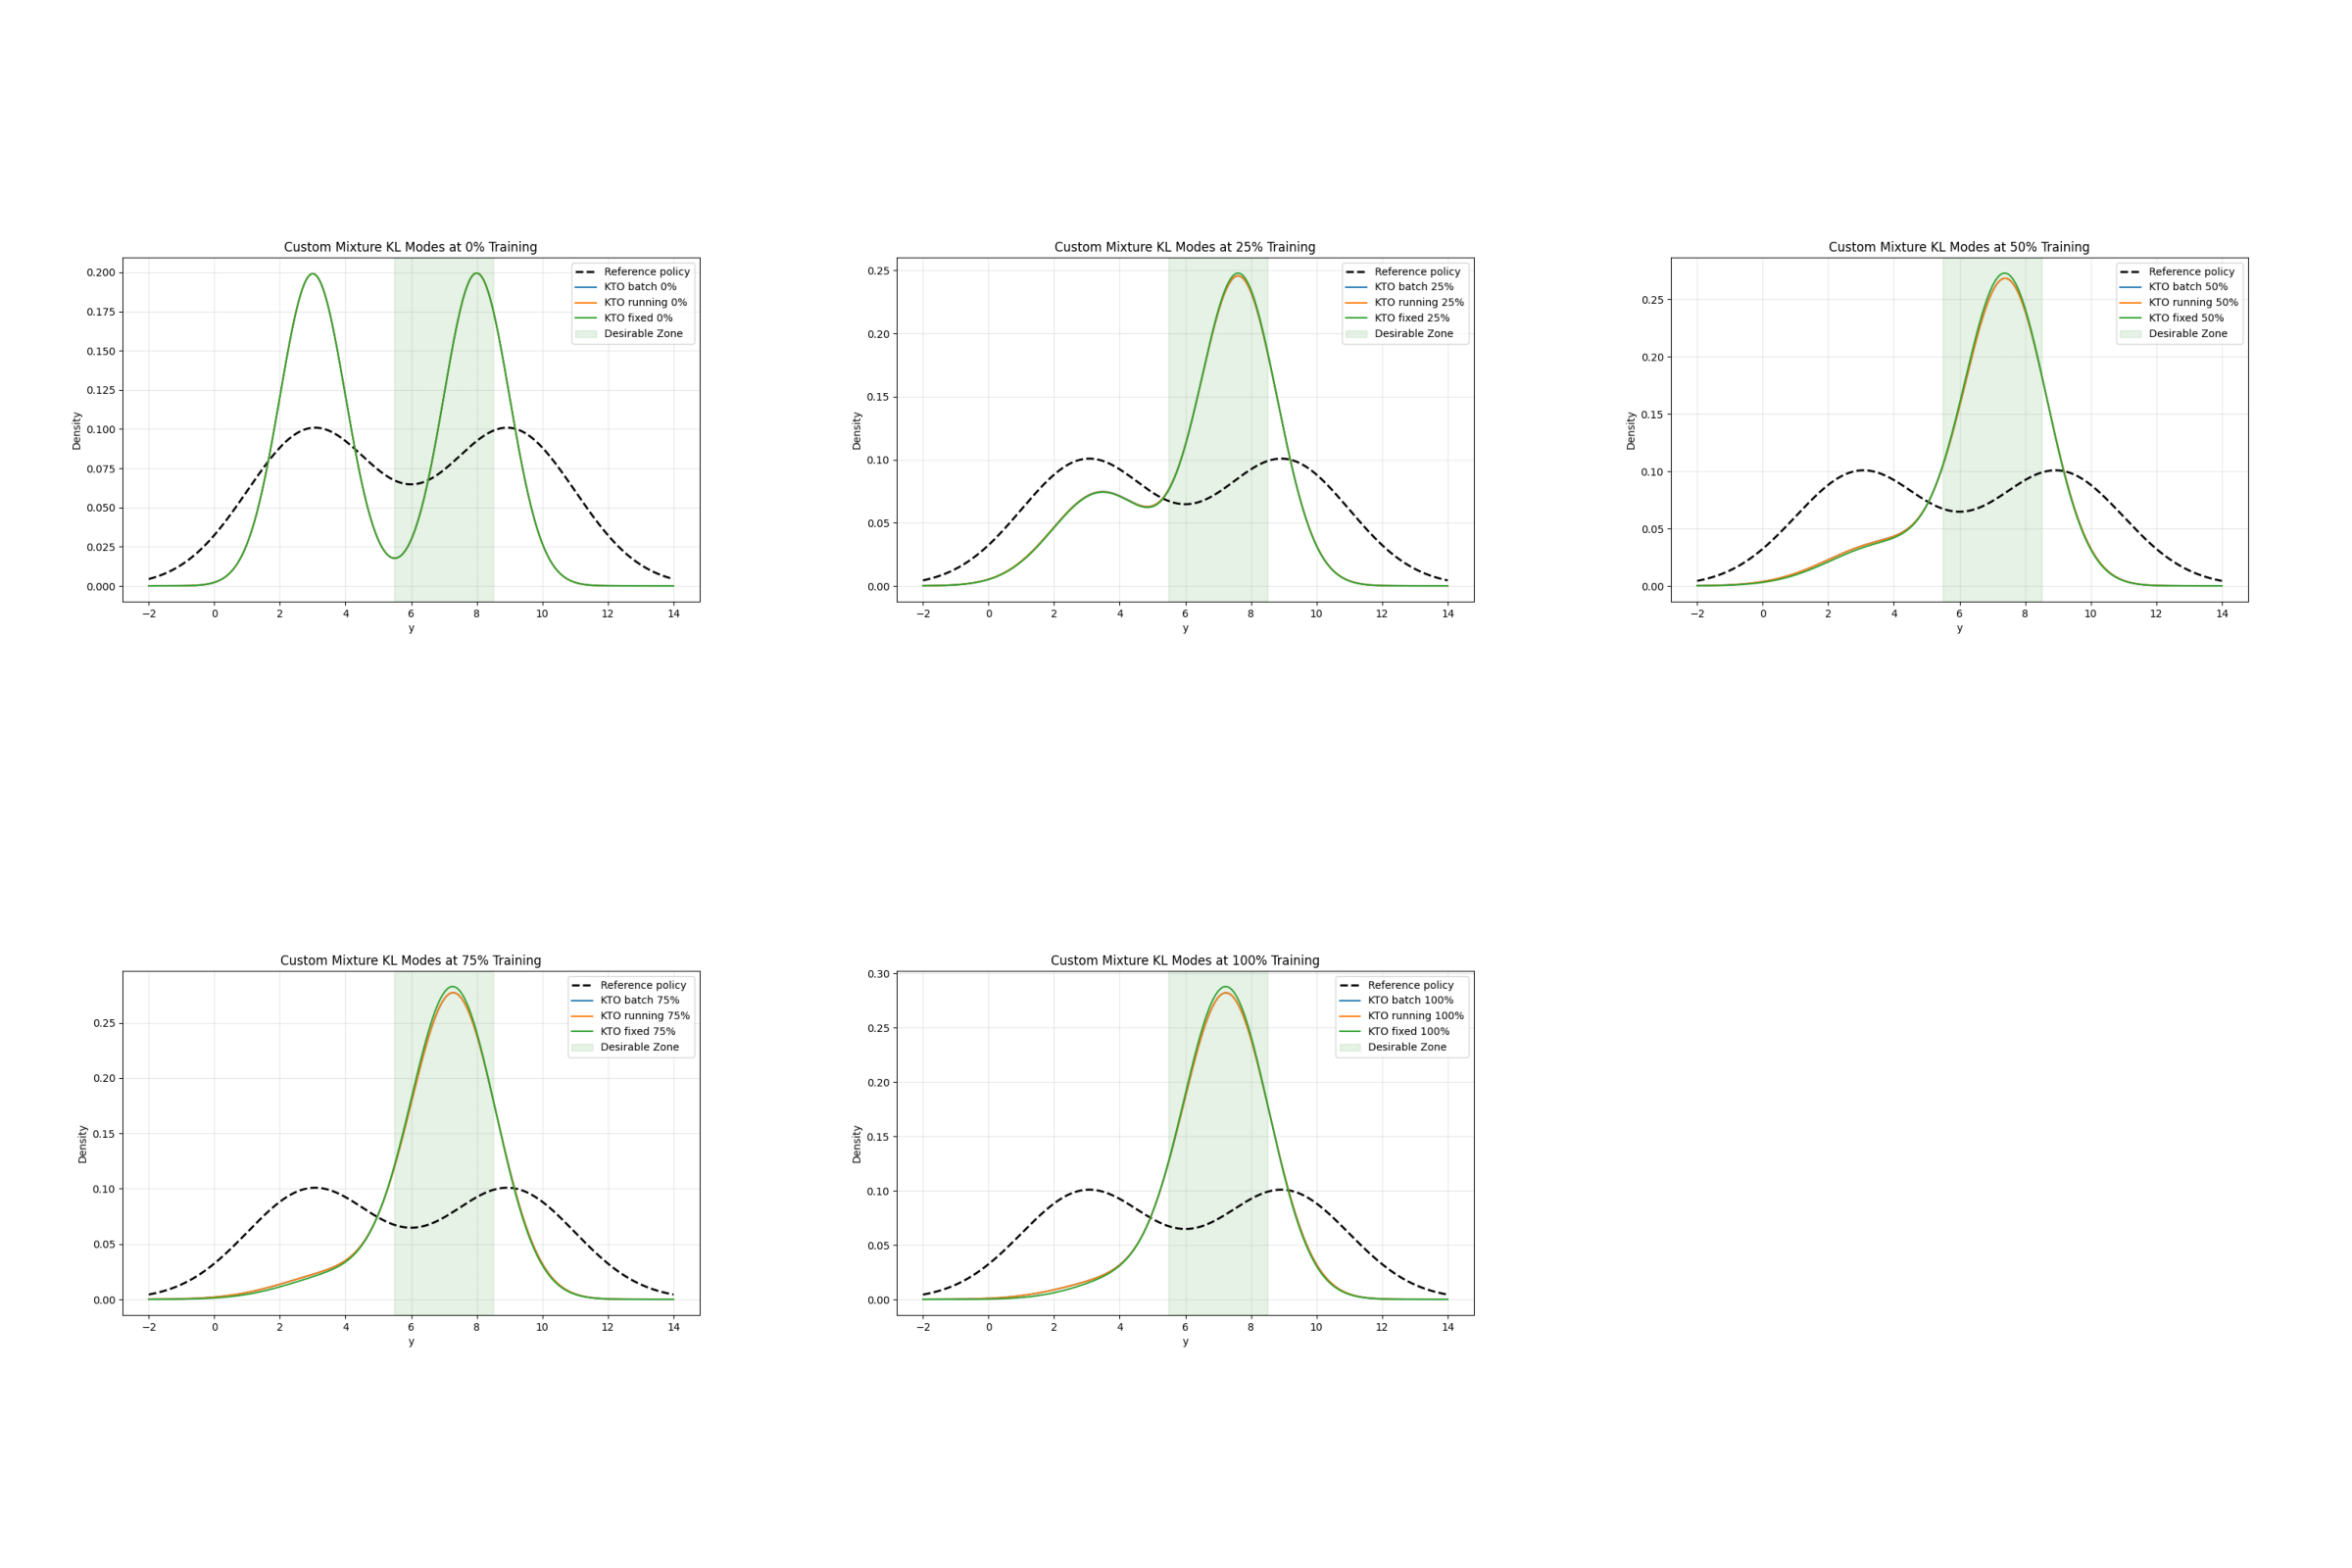
\includegraphics[width=0.95\textwidth]{figures/mix_reference_sampling_custom_montage.png}
    \caption{Custom mixture KL modes (quartiles).}
\end{figure}

\subsection{Component Entropy Dynamics}
\begin{figure}[H]
    \centering
    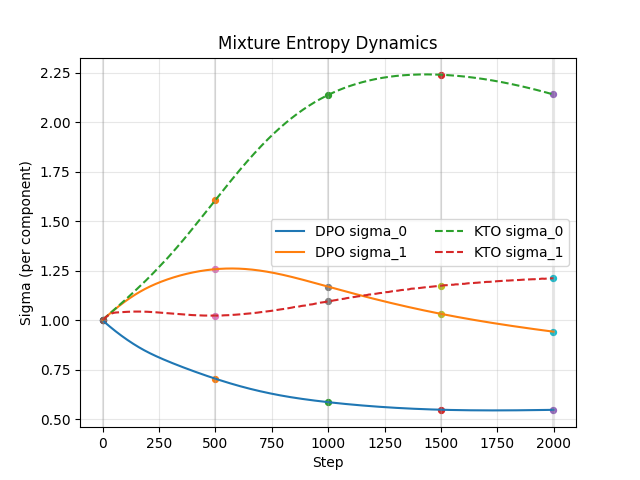
\includegraphics[width=0.9\textwidth]{figures/mix_entropy_dynamics.png}
    \caption{Per-component sigma dynamics for mixture DPO vs KTO.}
\end{figure}

\section{Mixture Initialization Sensitivity and Weight Selection}
\begin{figure}[H]
    \centering
    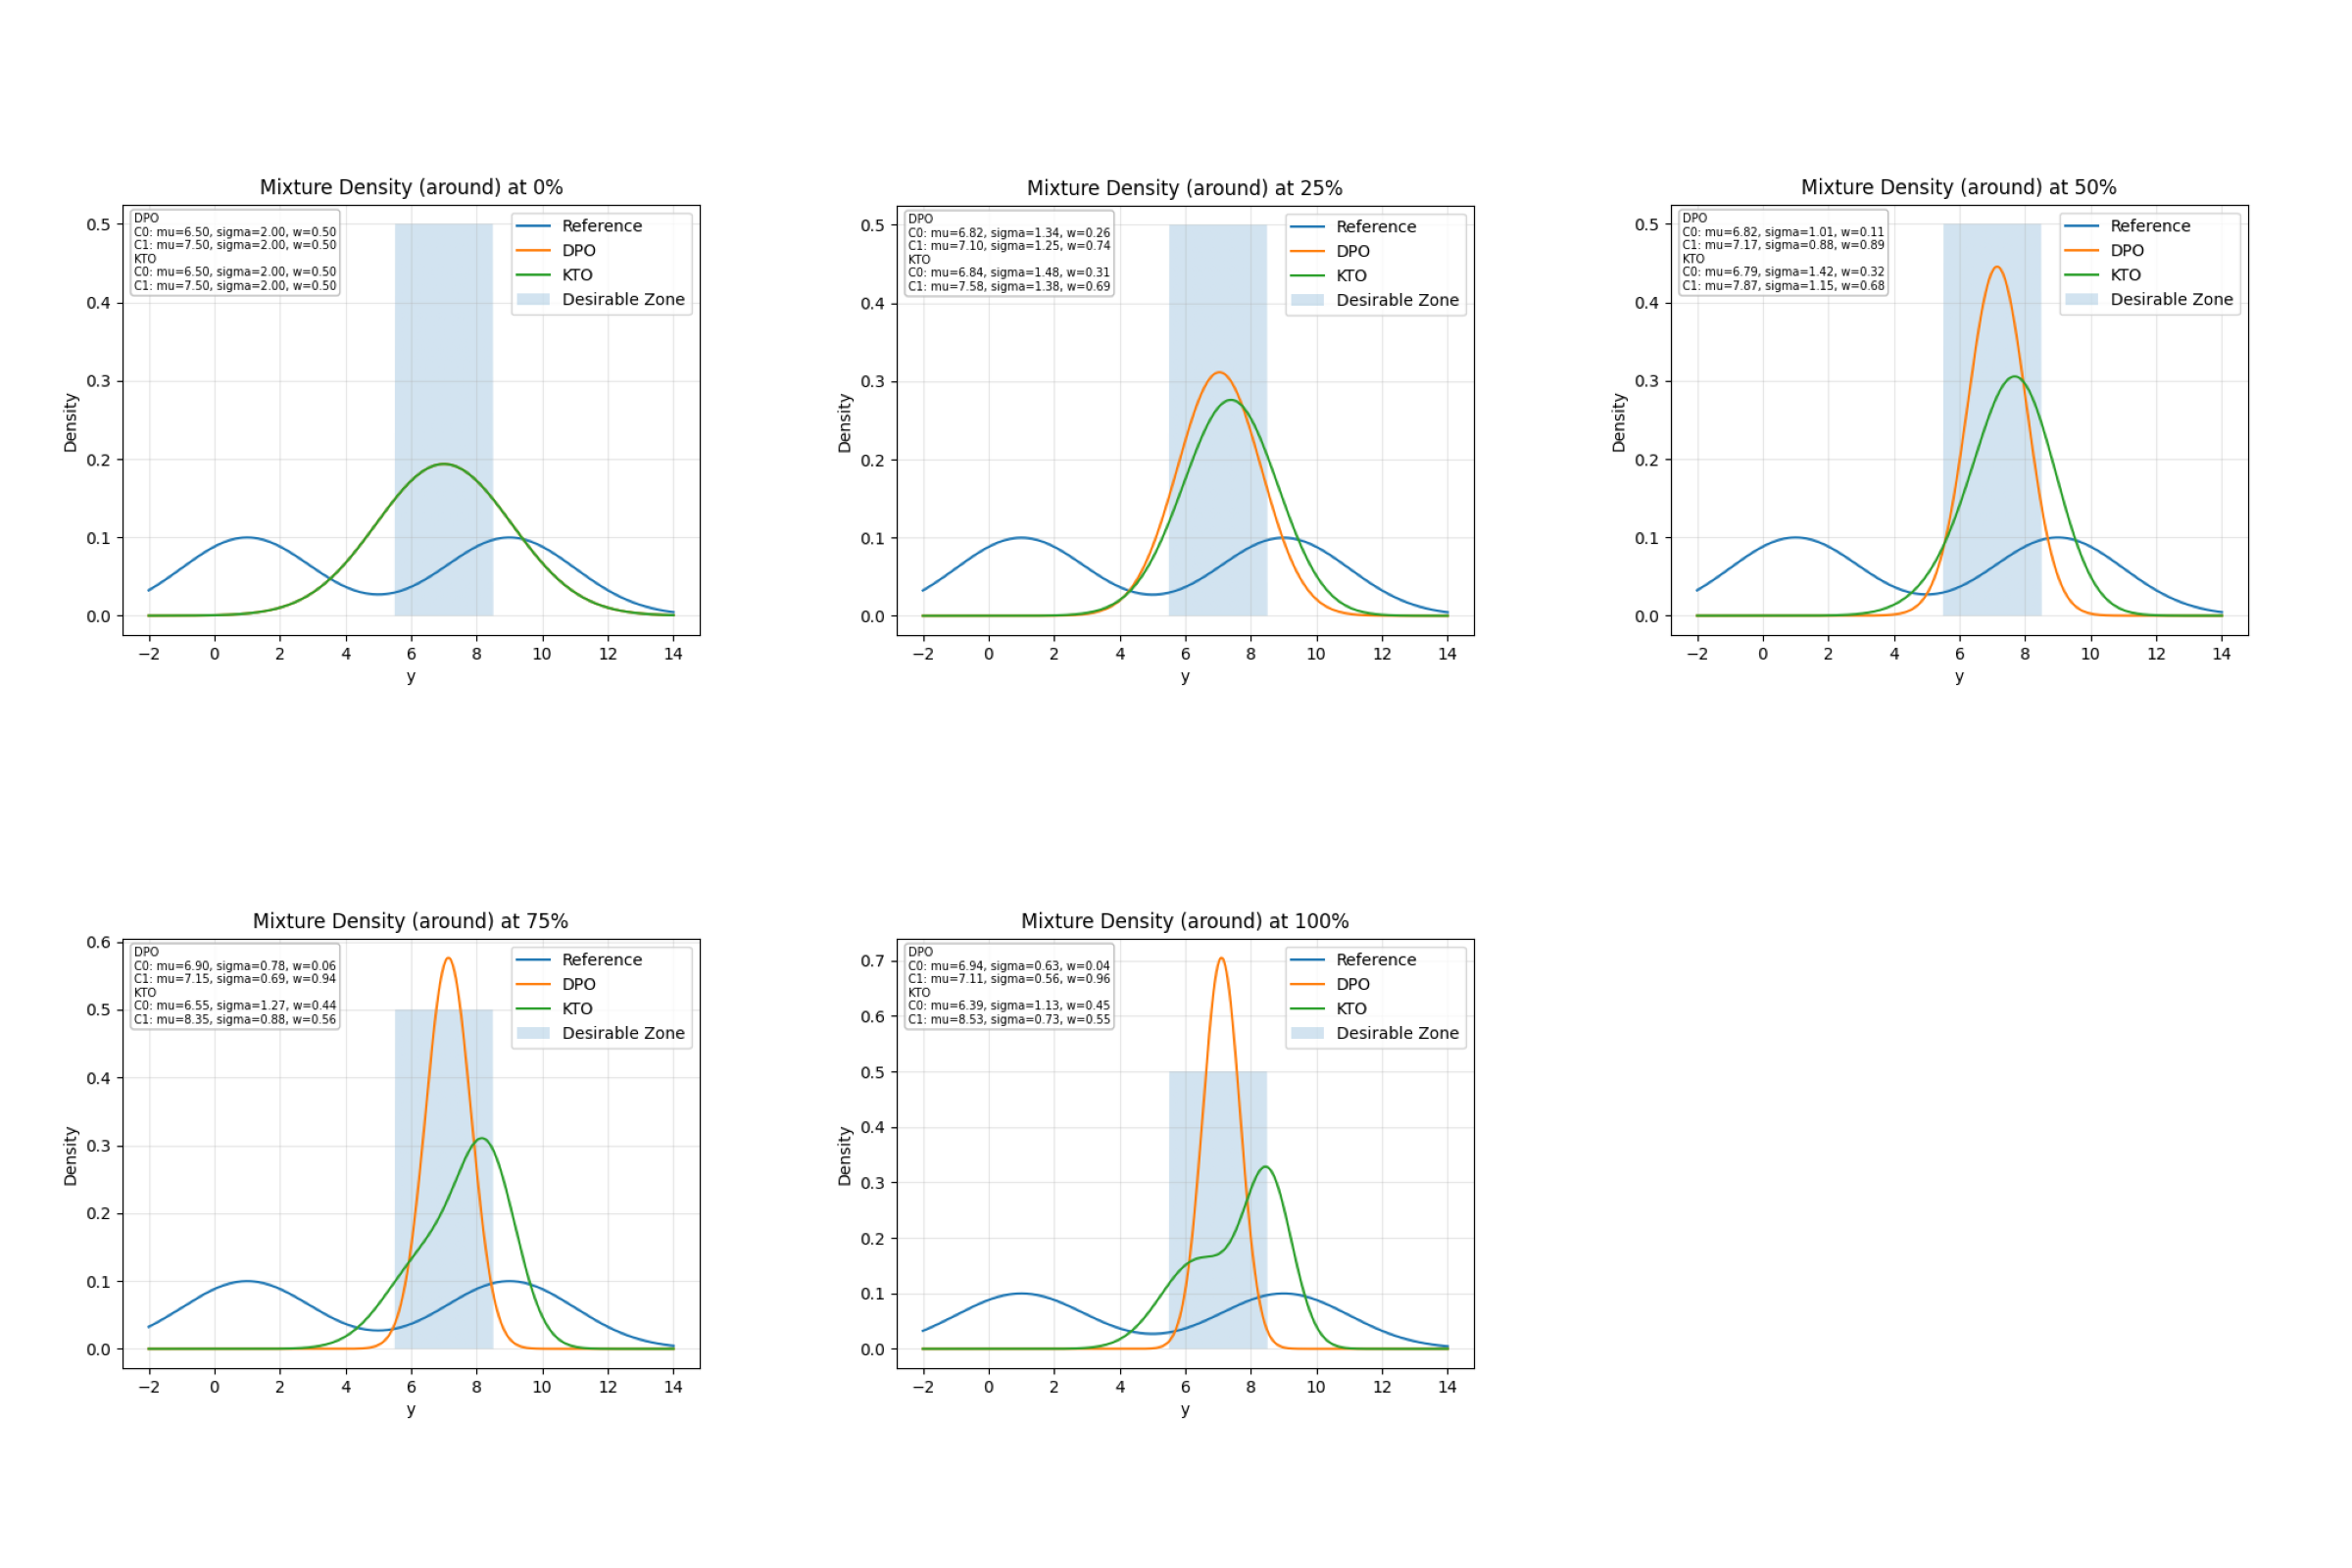
\includegraphics[width=0.95\textwidth]{figures/mix_init_density_around.png}
    \caption{Mixture init around 7: density evolution montage.}
\end{figure}

\begin{figure}[H]
    \centering
    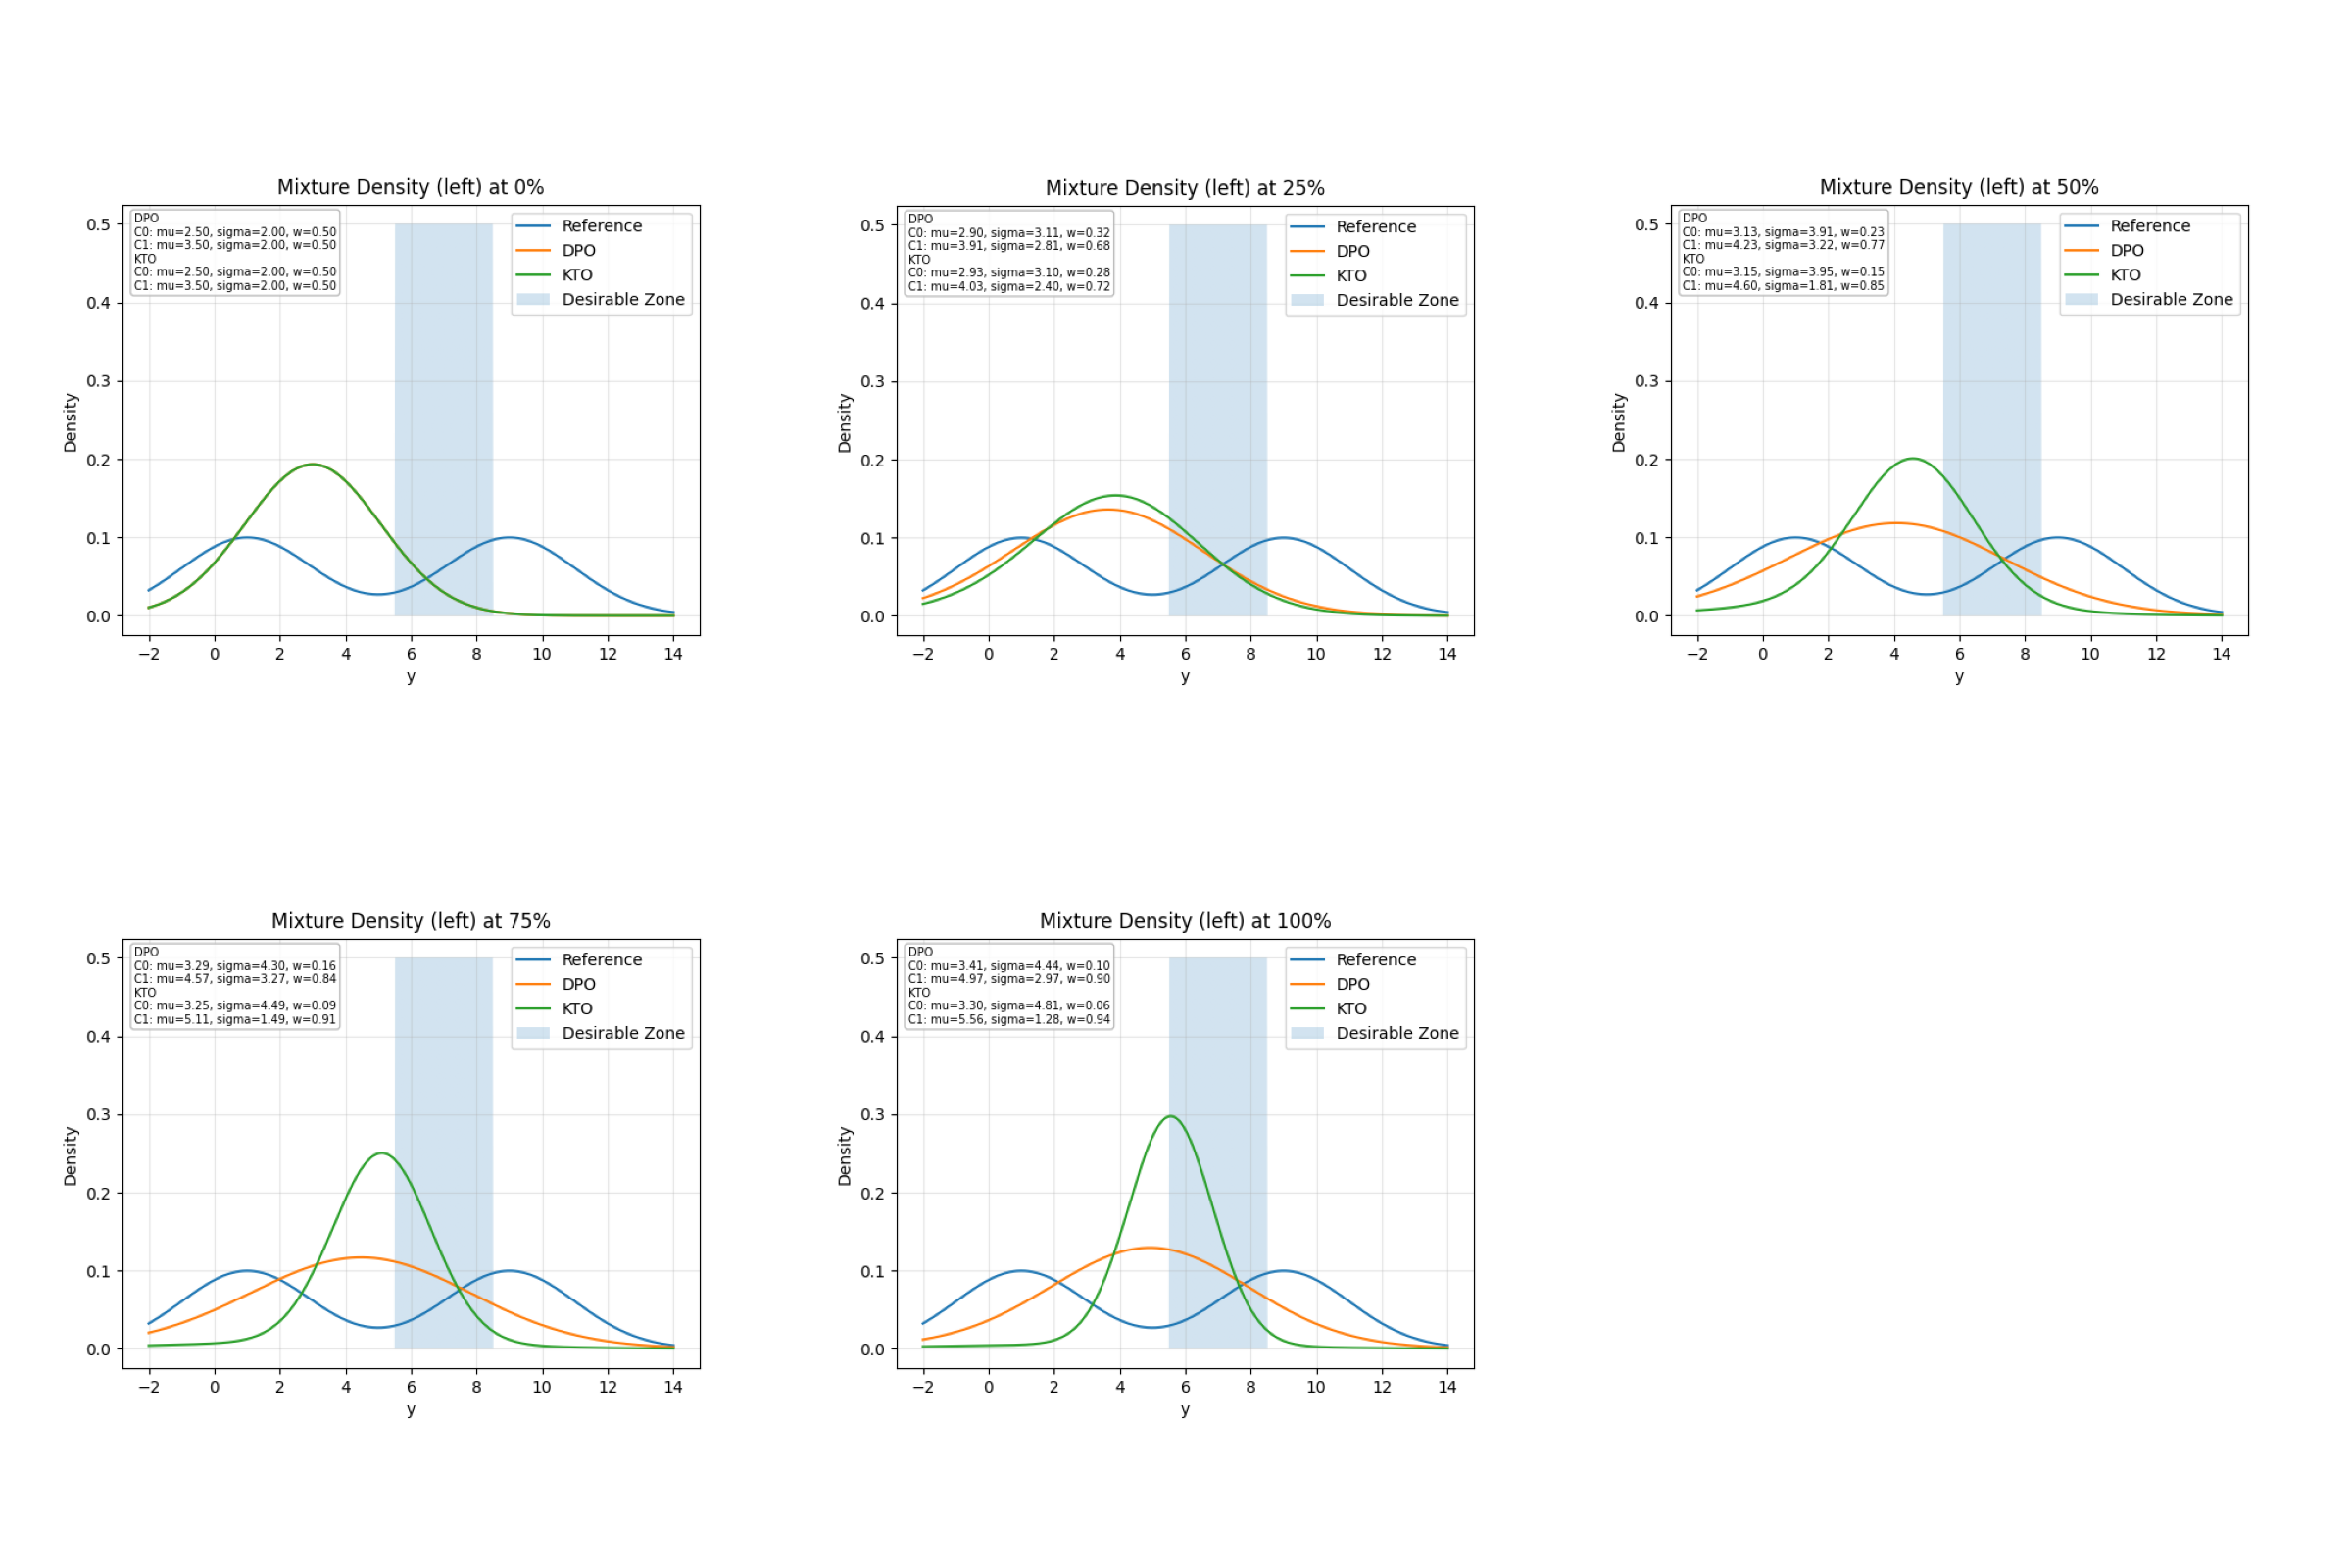
\includegraphics[width=0.95\textwidth]{figures/mix_init_density_left.png}
    \caption{Mixture init left of 7: density evolution montage.}
\end{figure}

\begin{figure}[H]
    \centering
    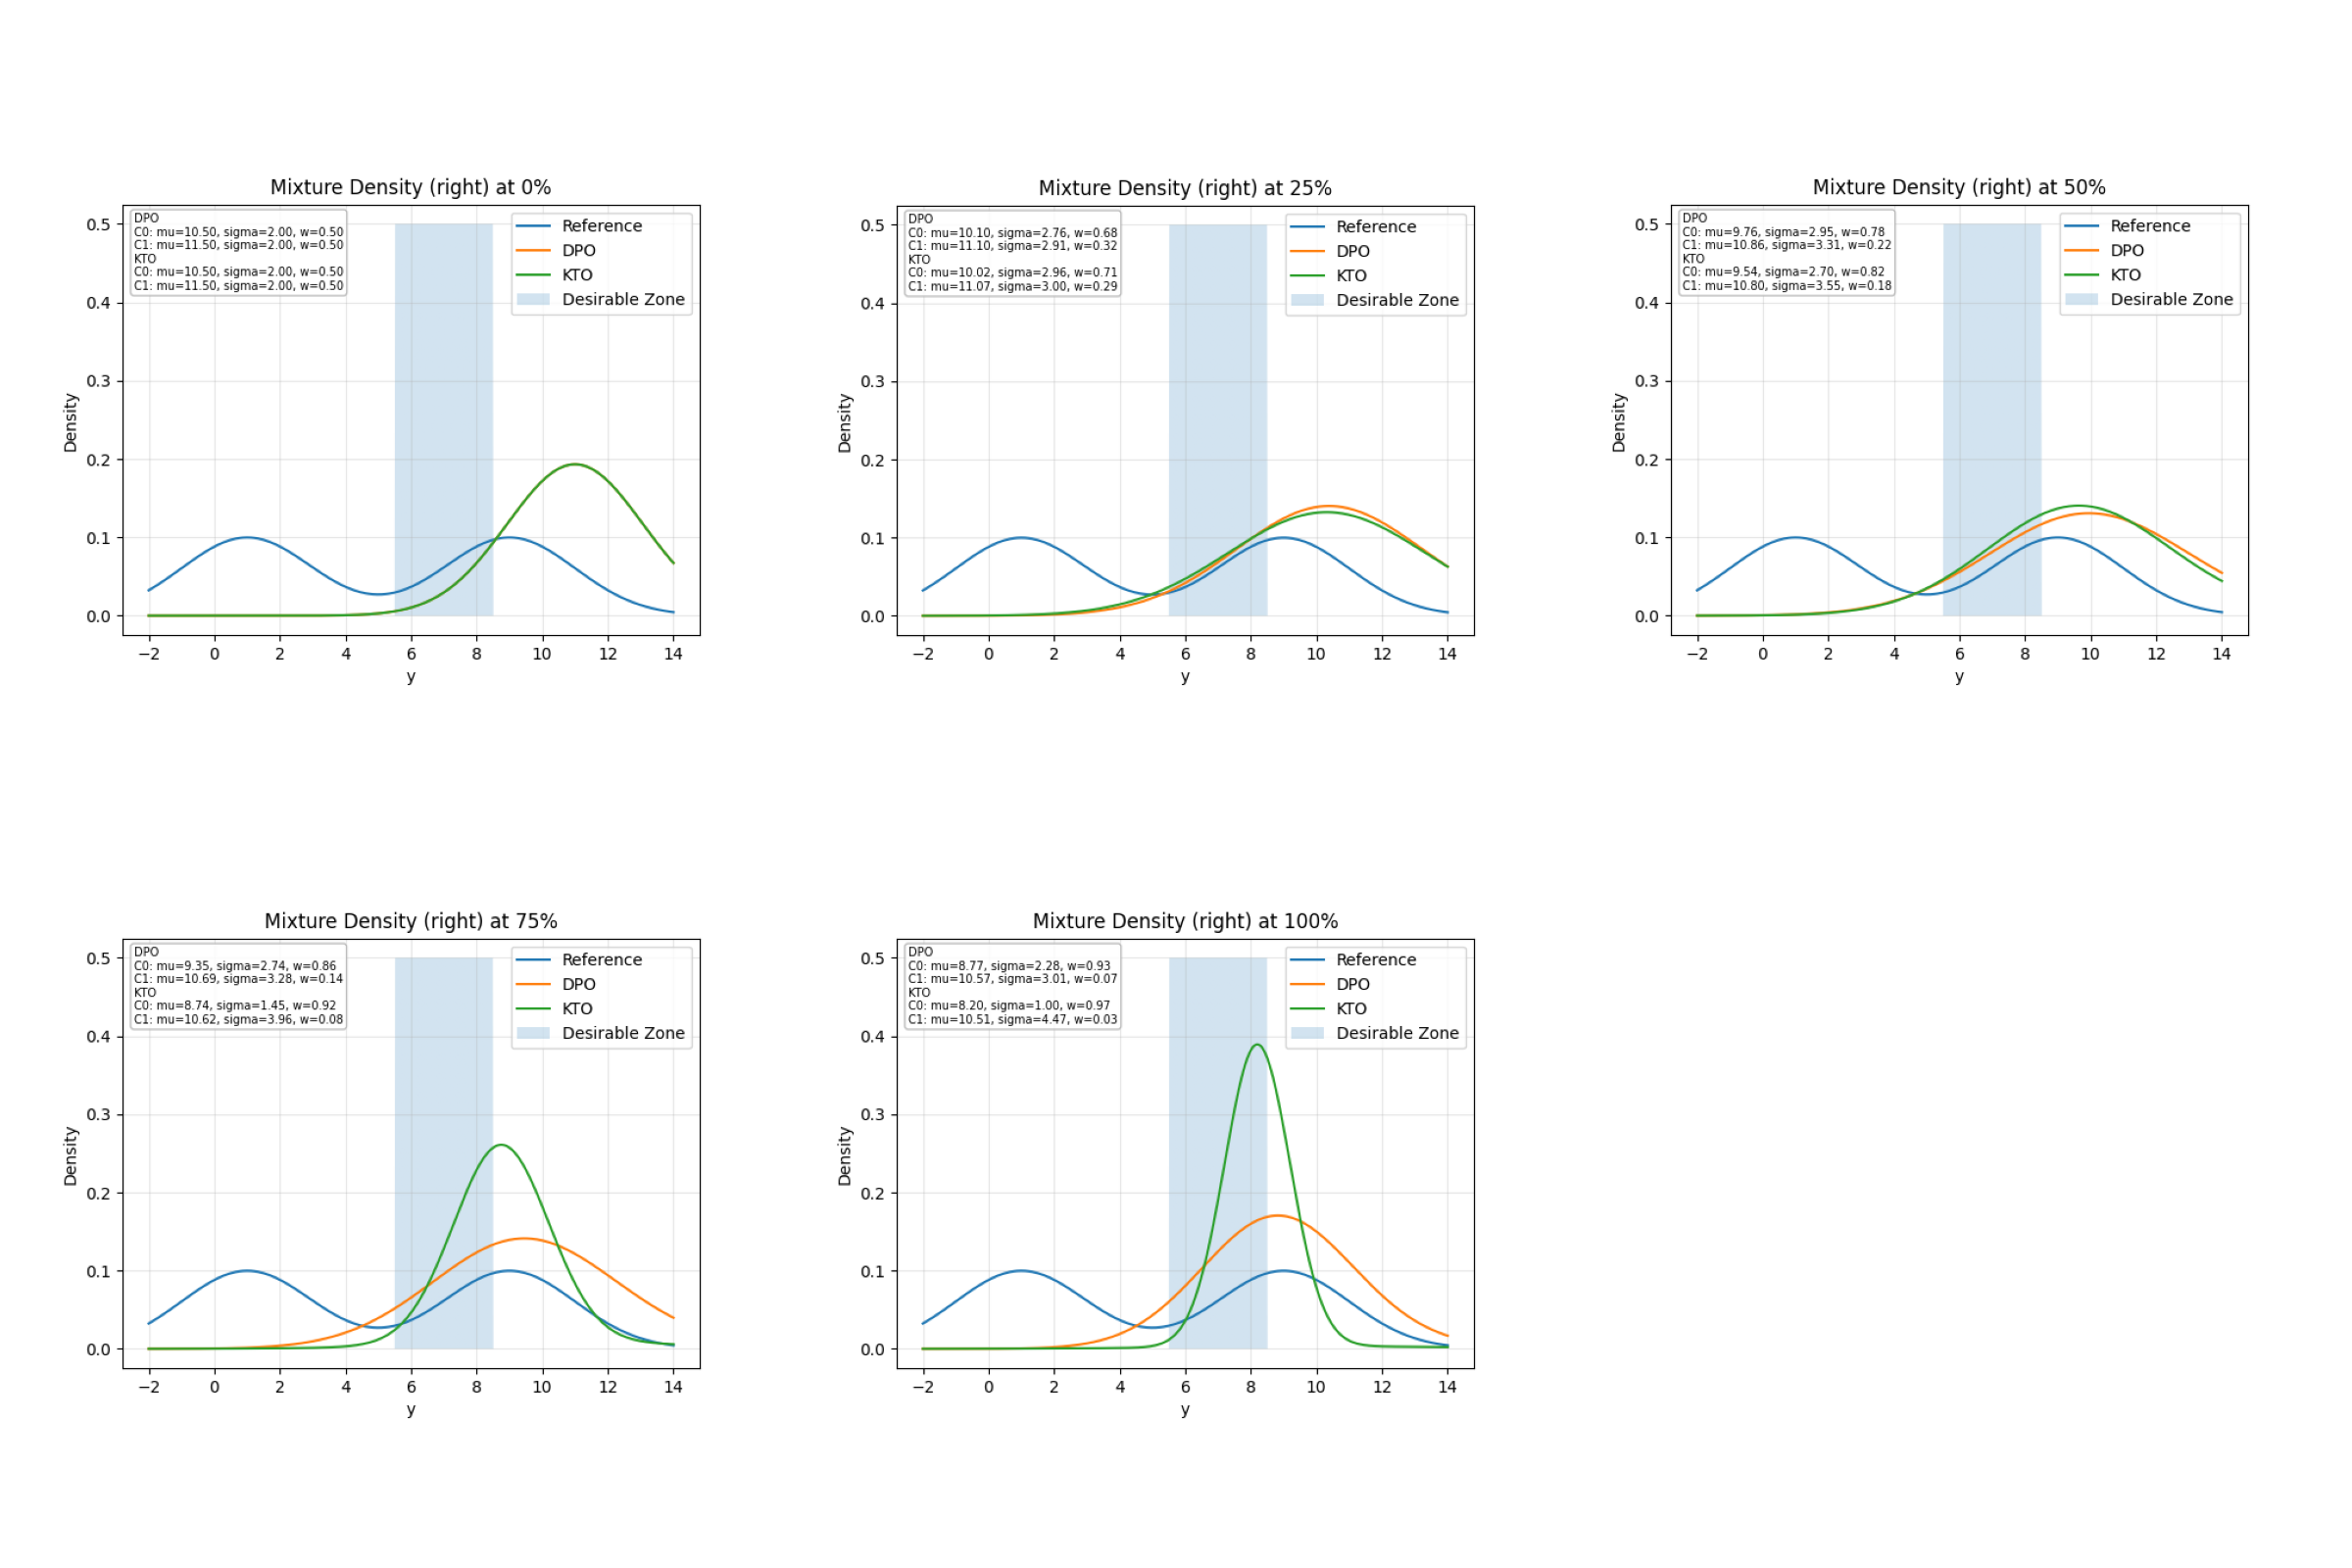
\includegraphics[width=0.95\textwidth]{figures/mix_init_density_right.png}
    \caption{Mixture init right of 7: density evolution montage.}
\end{figure}

\begin{figure}[H]
    \centering
    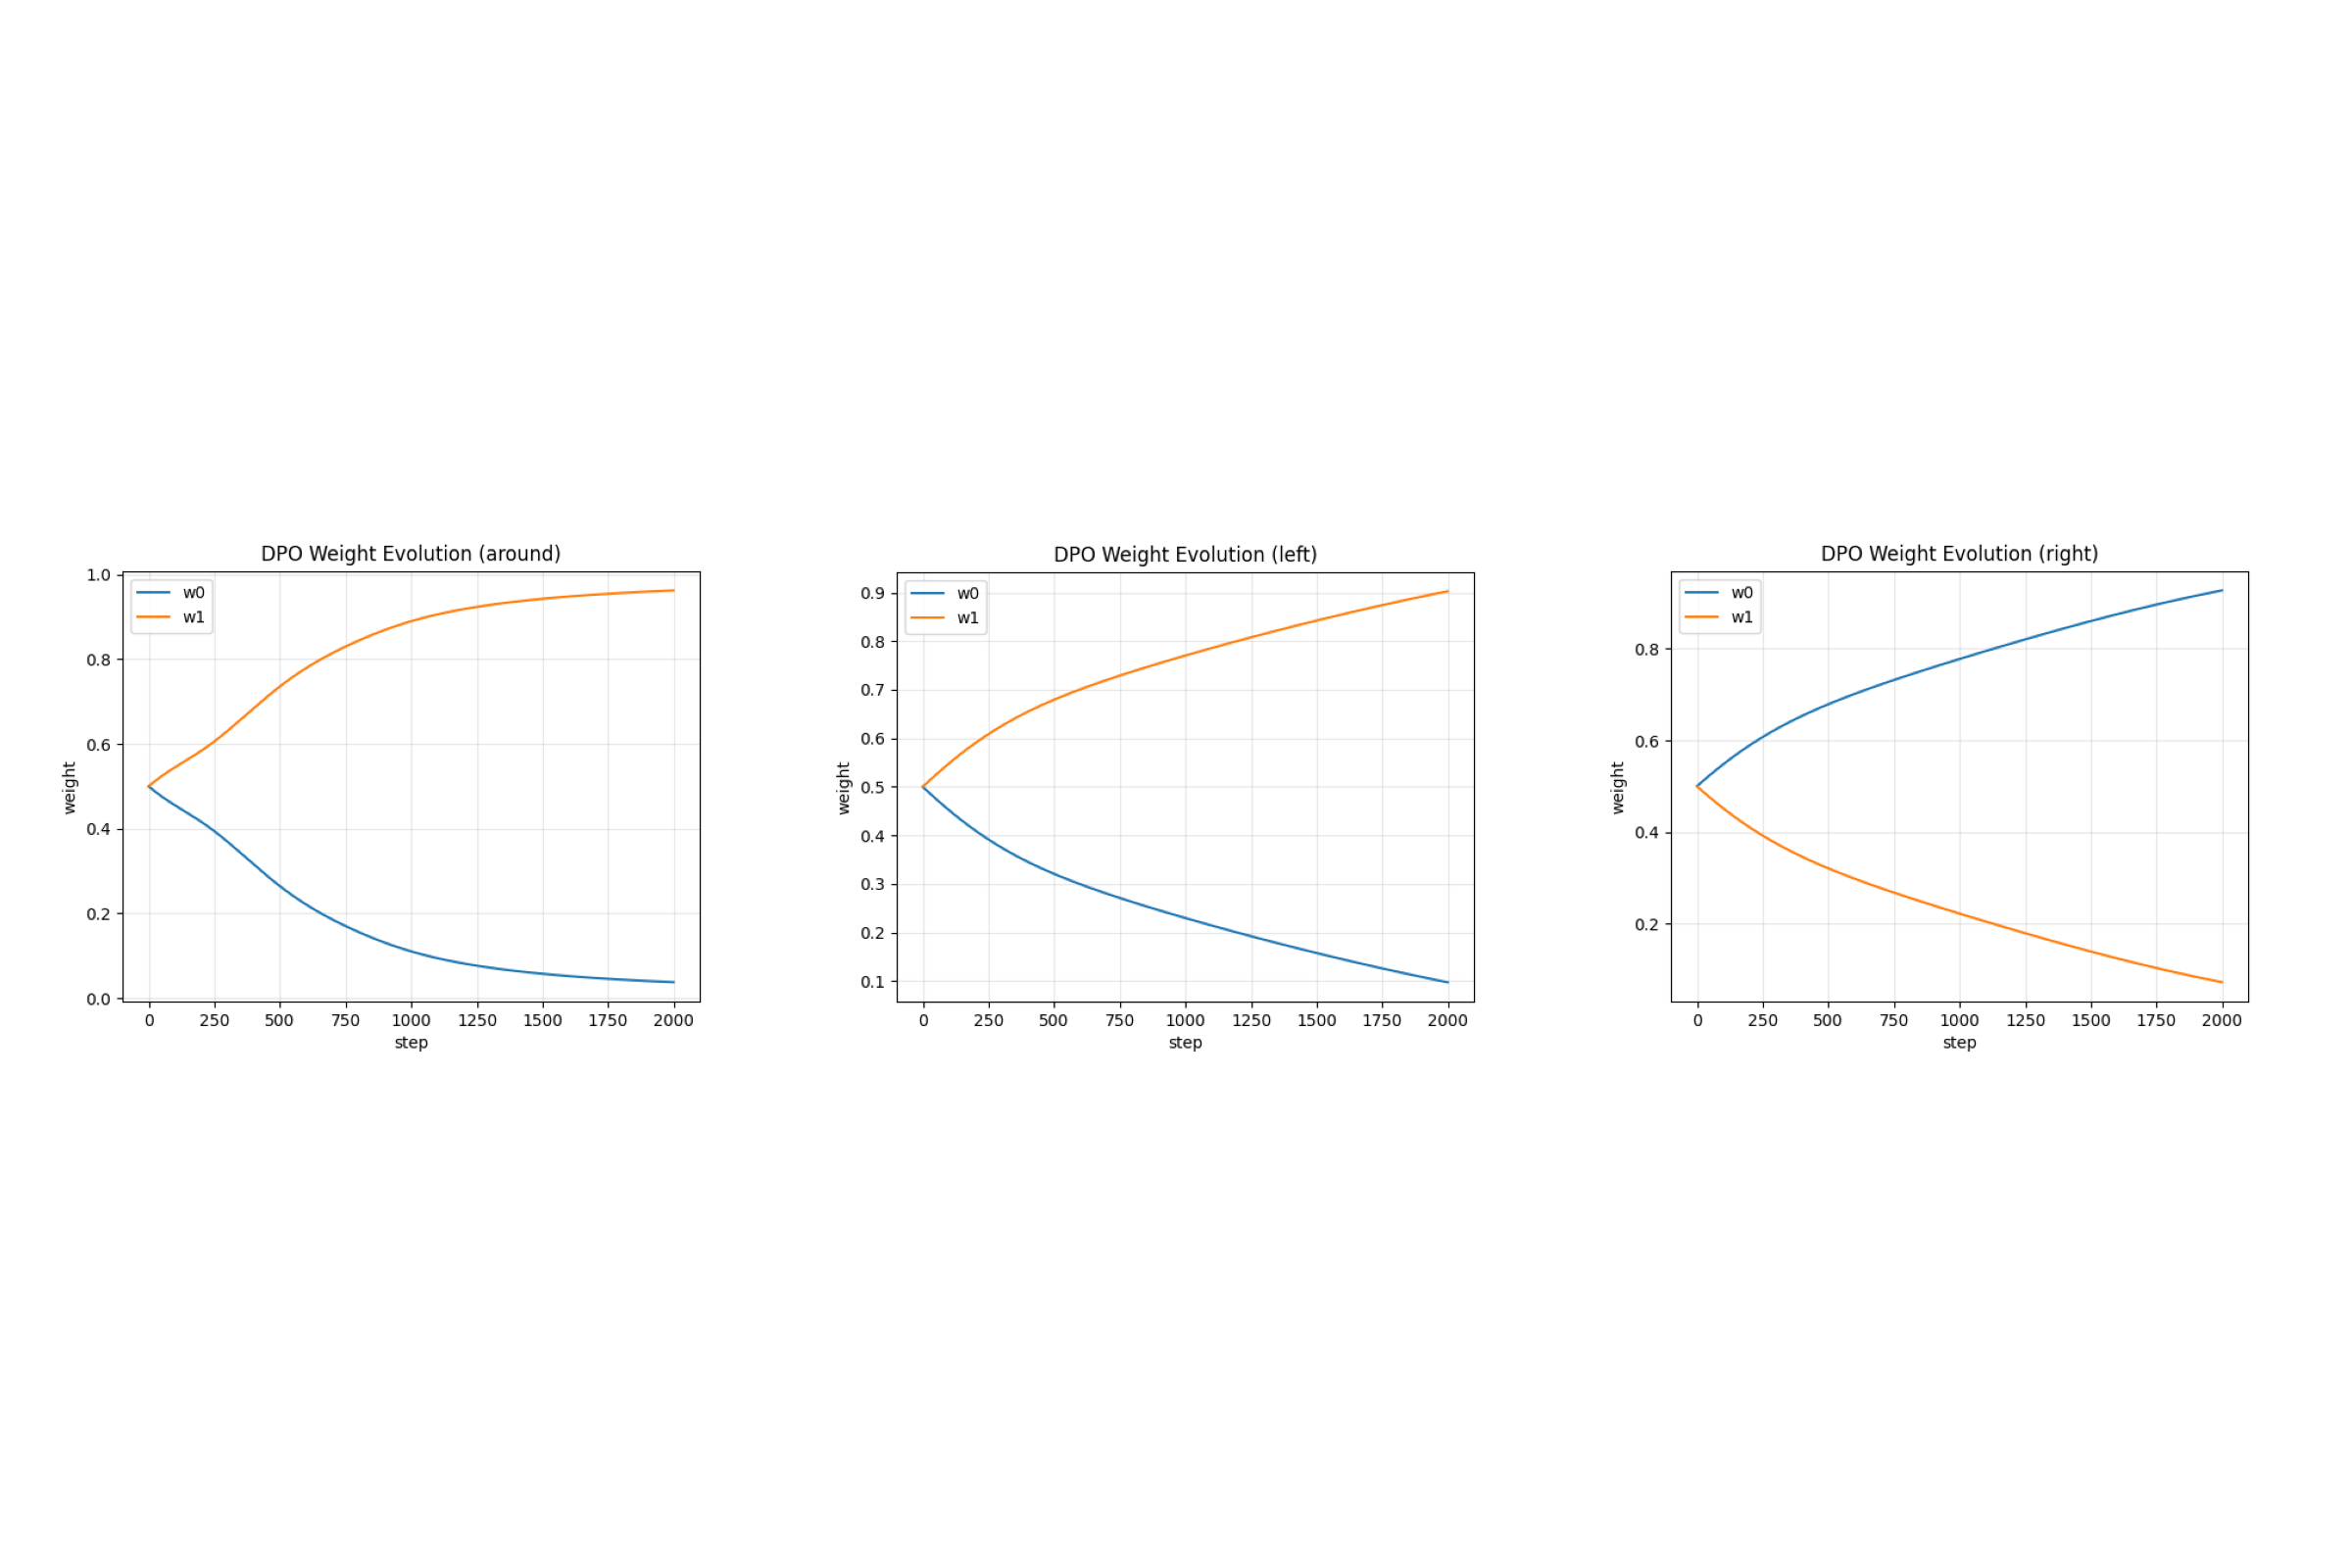
\includegraphics[width=0.9\textwidth]{figures/mix_dpo_weights_montage.png}
    \caption{DPO mixture weight evolution (around/left/right).}
\end{figure}

\begin{figure}[H]
    \centering
    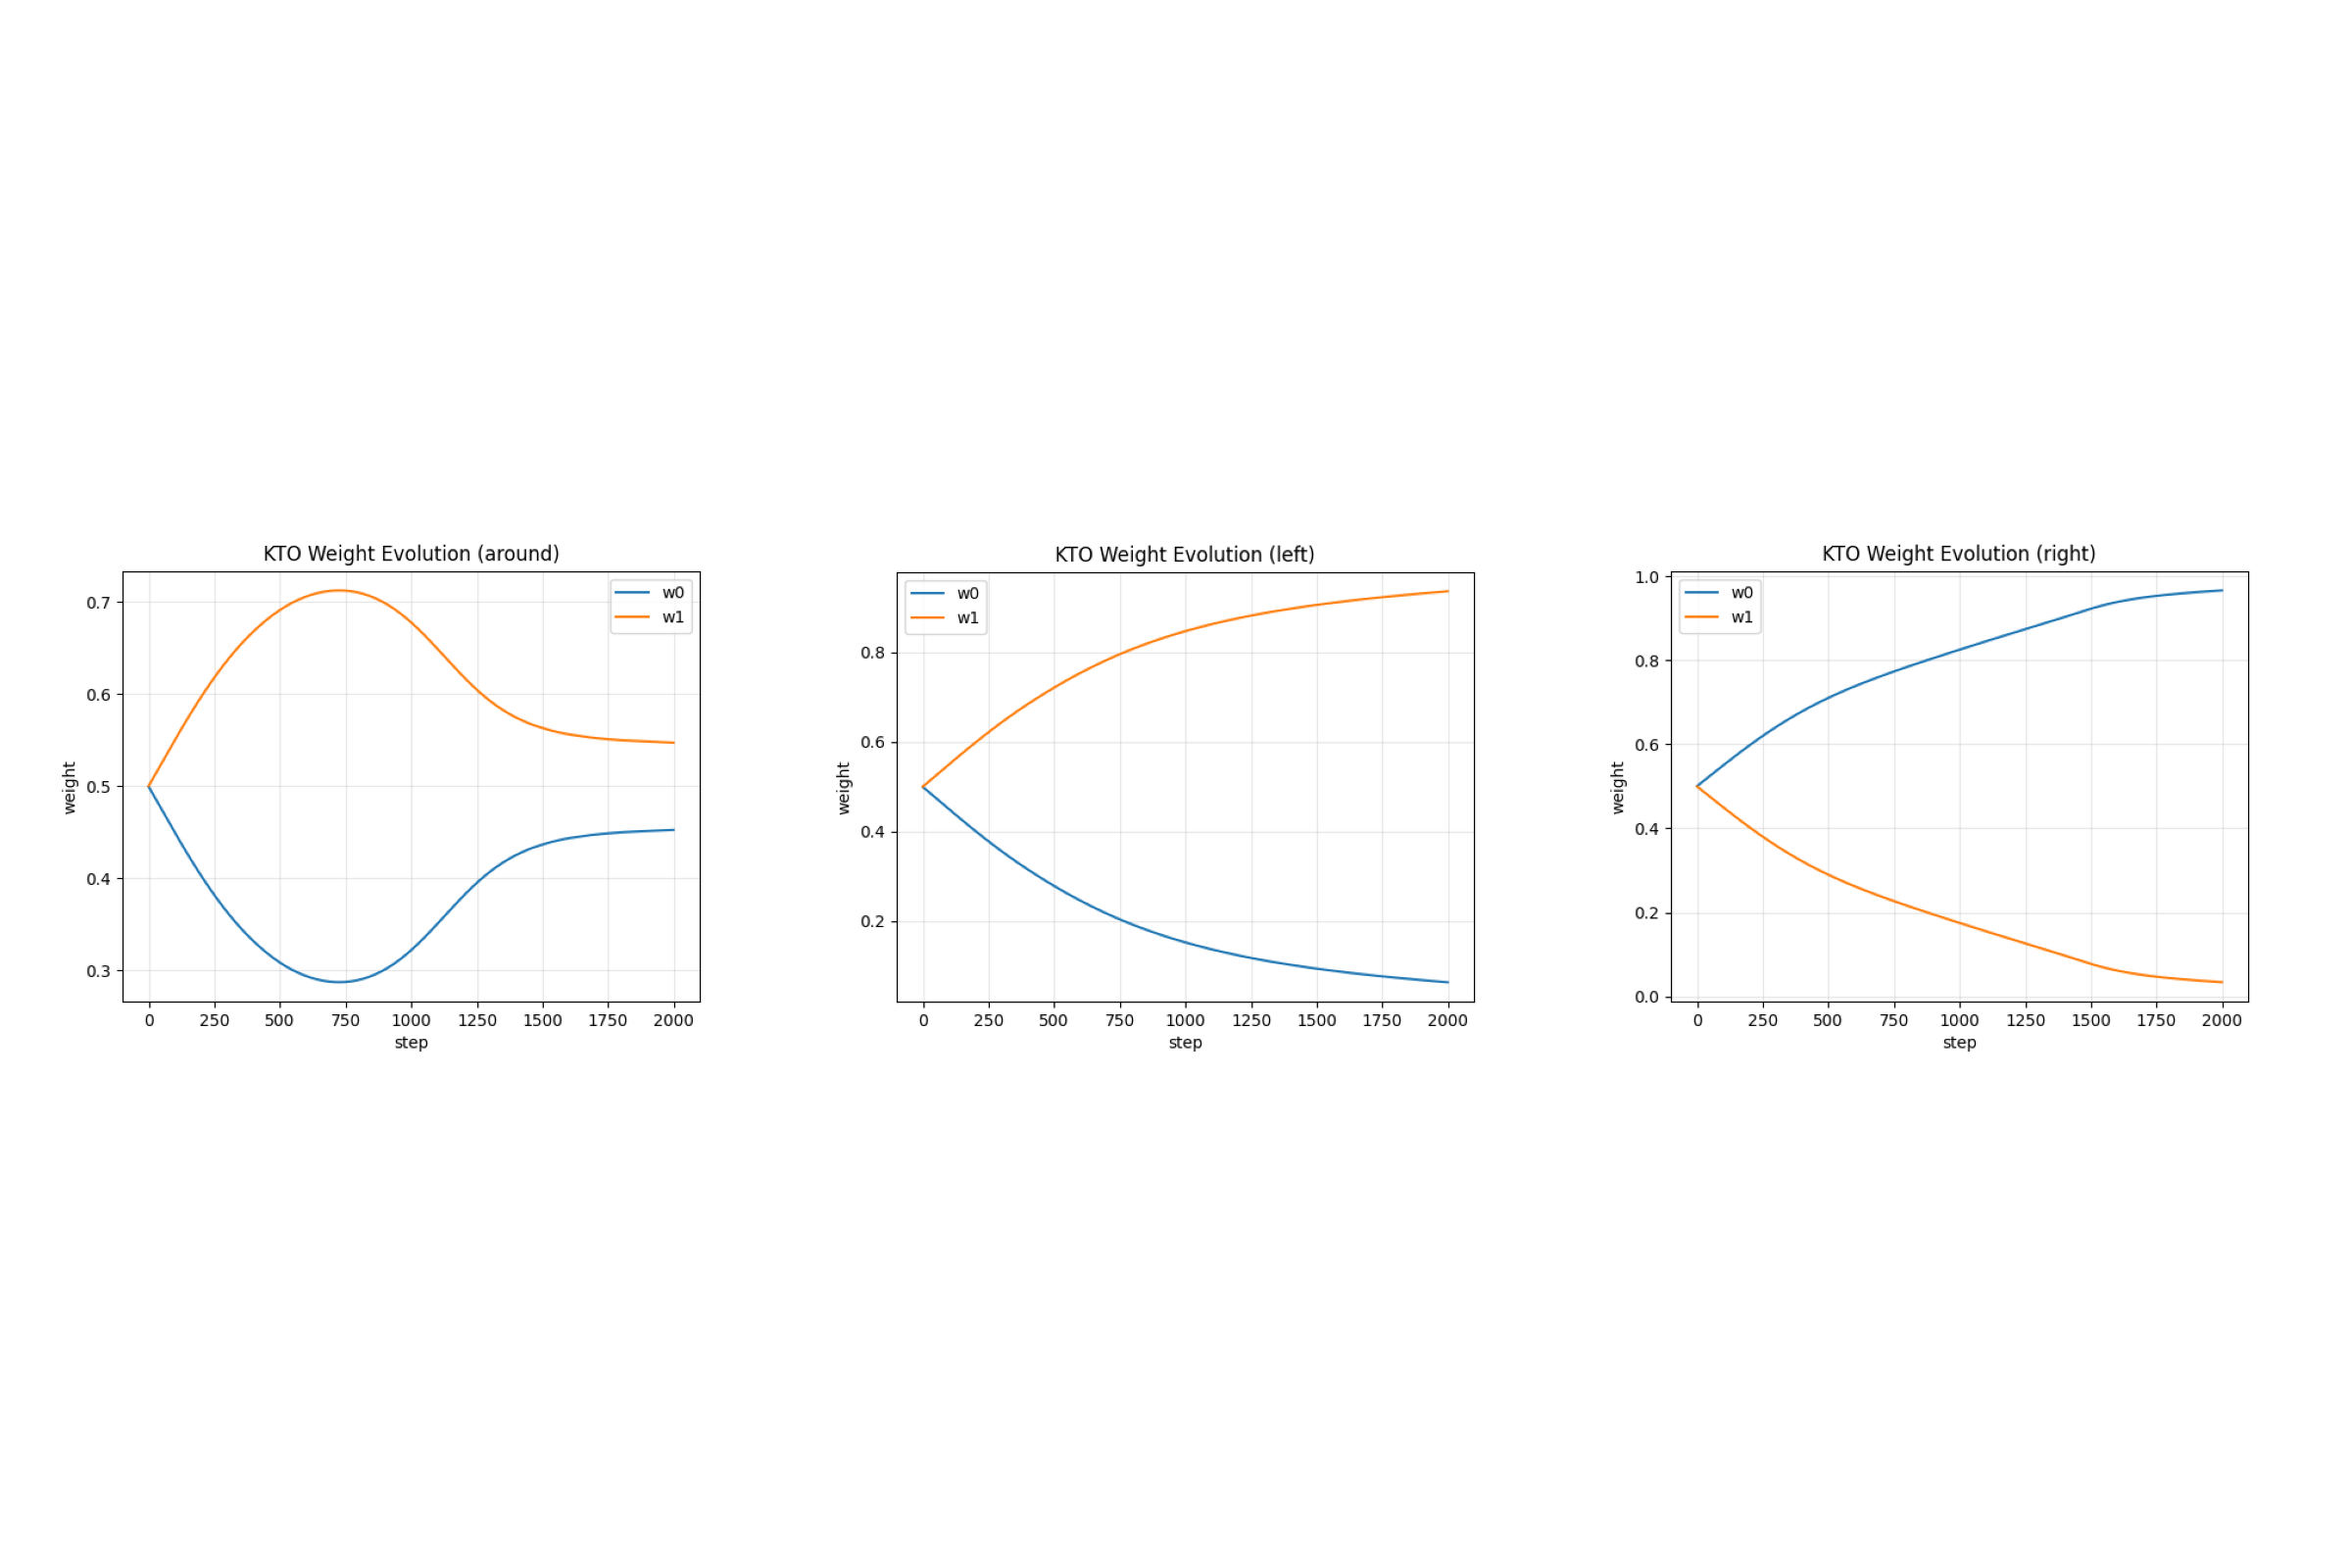
\includegraphics[width=0.9\textwidth]{figures/mix_kto_weights_montage.png}
    \caption{KTO mixture weight evolution (around/left/right).}
\end{figure}

\section{New: Mixture Component Evolution and Milestones}
\begin{figure}[H]
    \centering
    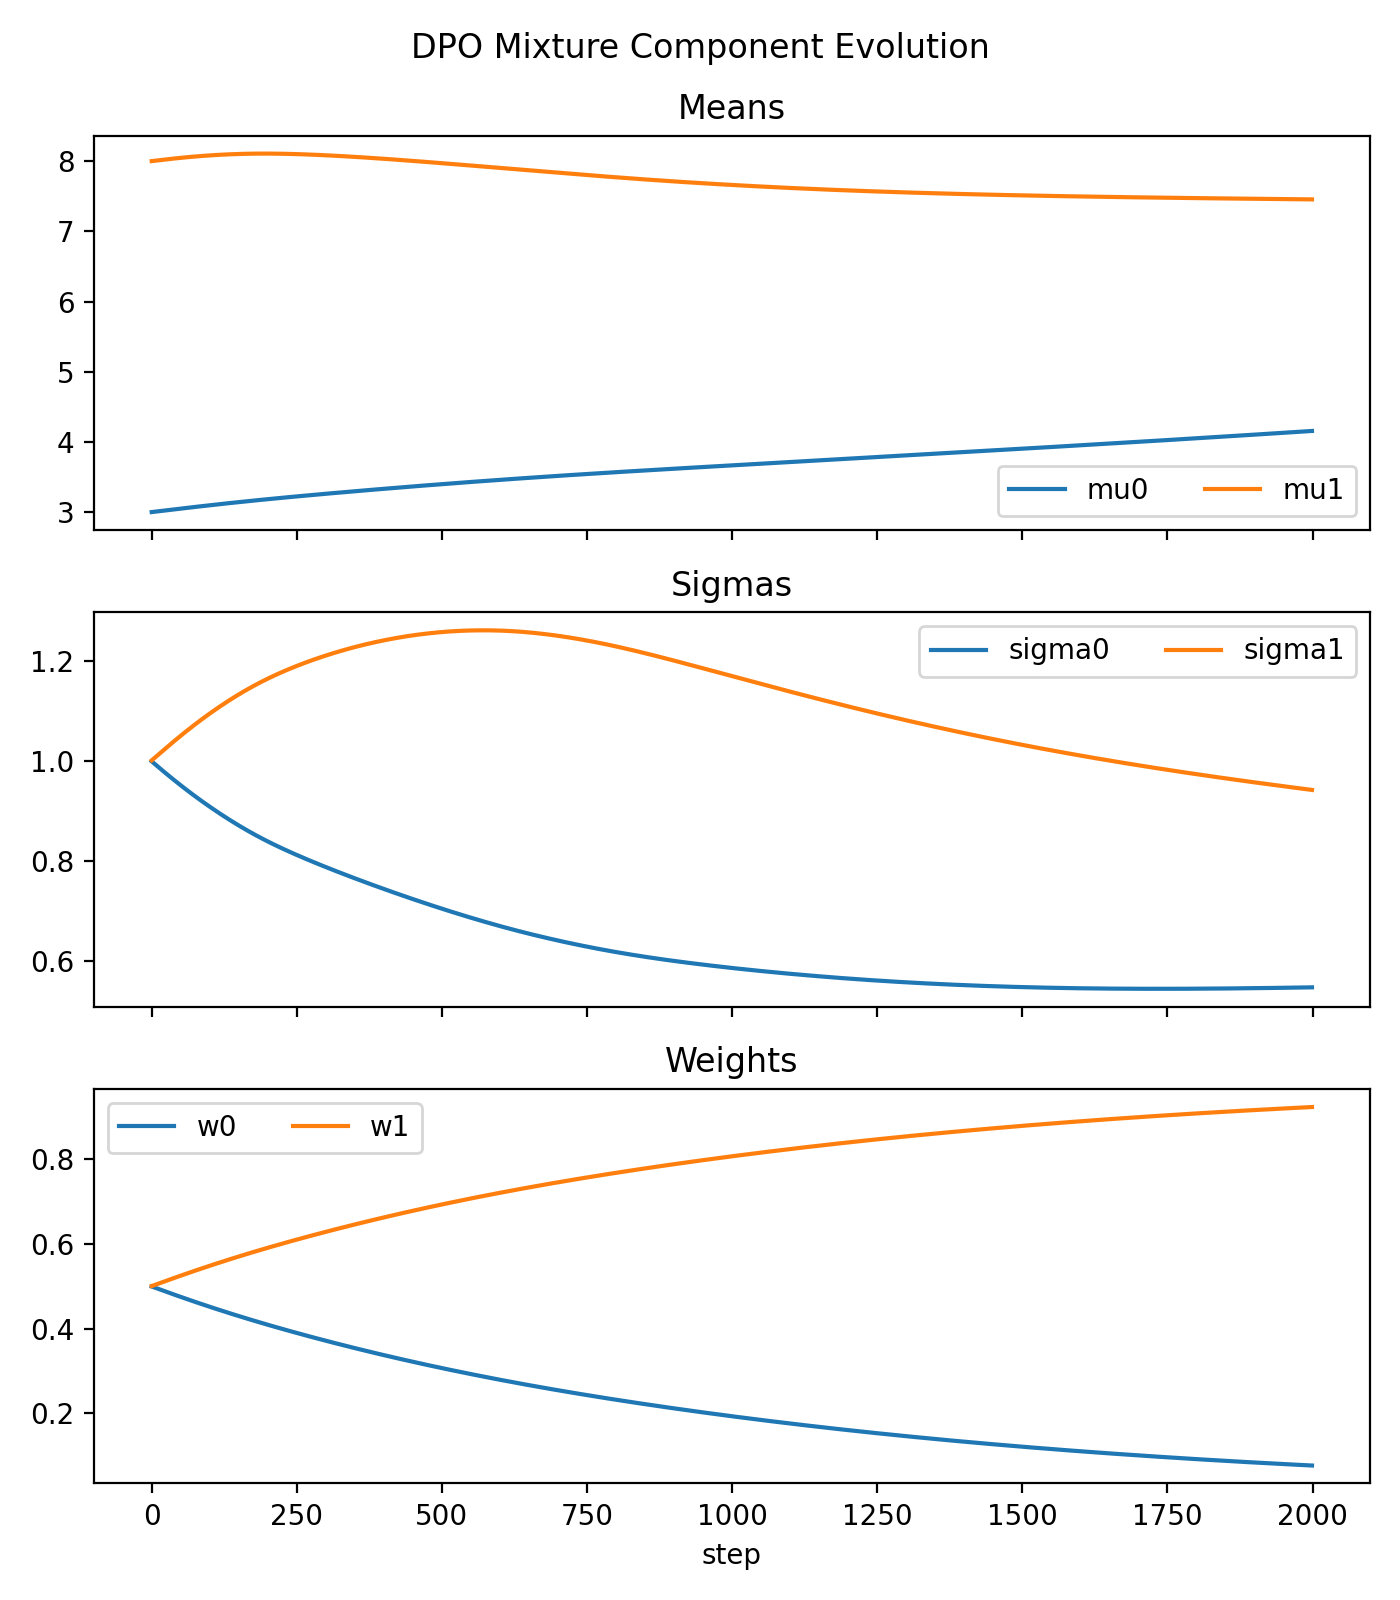
\includegraphics[width=0.95\textwidth]{figures/mix_component_evolution_dpo.png}
    \caption{DPO mixture component evolution (mu, sigma, weights).}
\end{figure}

\begin{figure}[H]
    \centering
    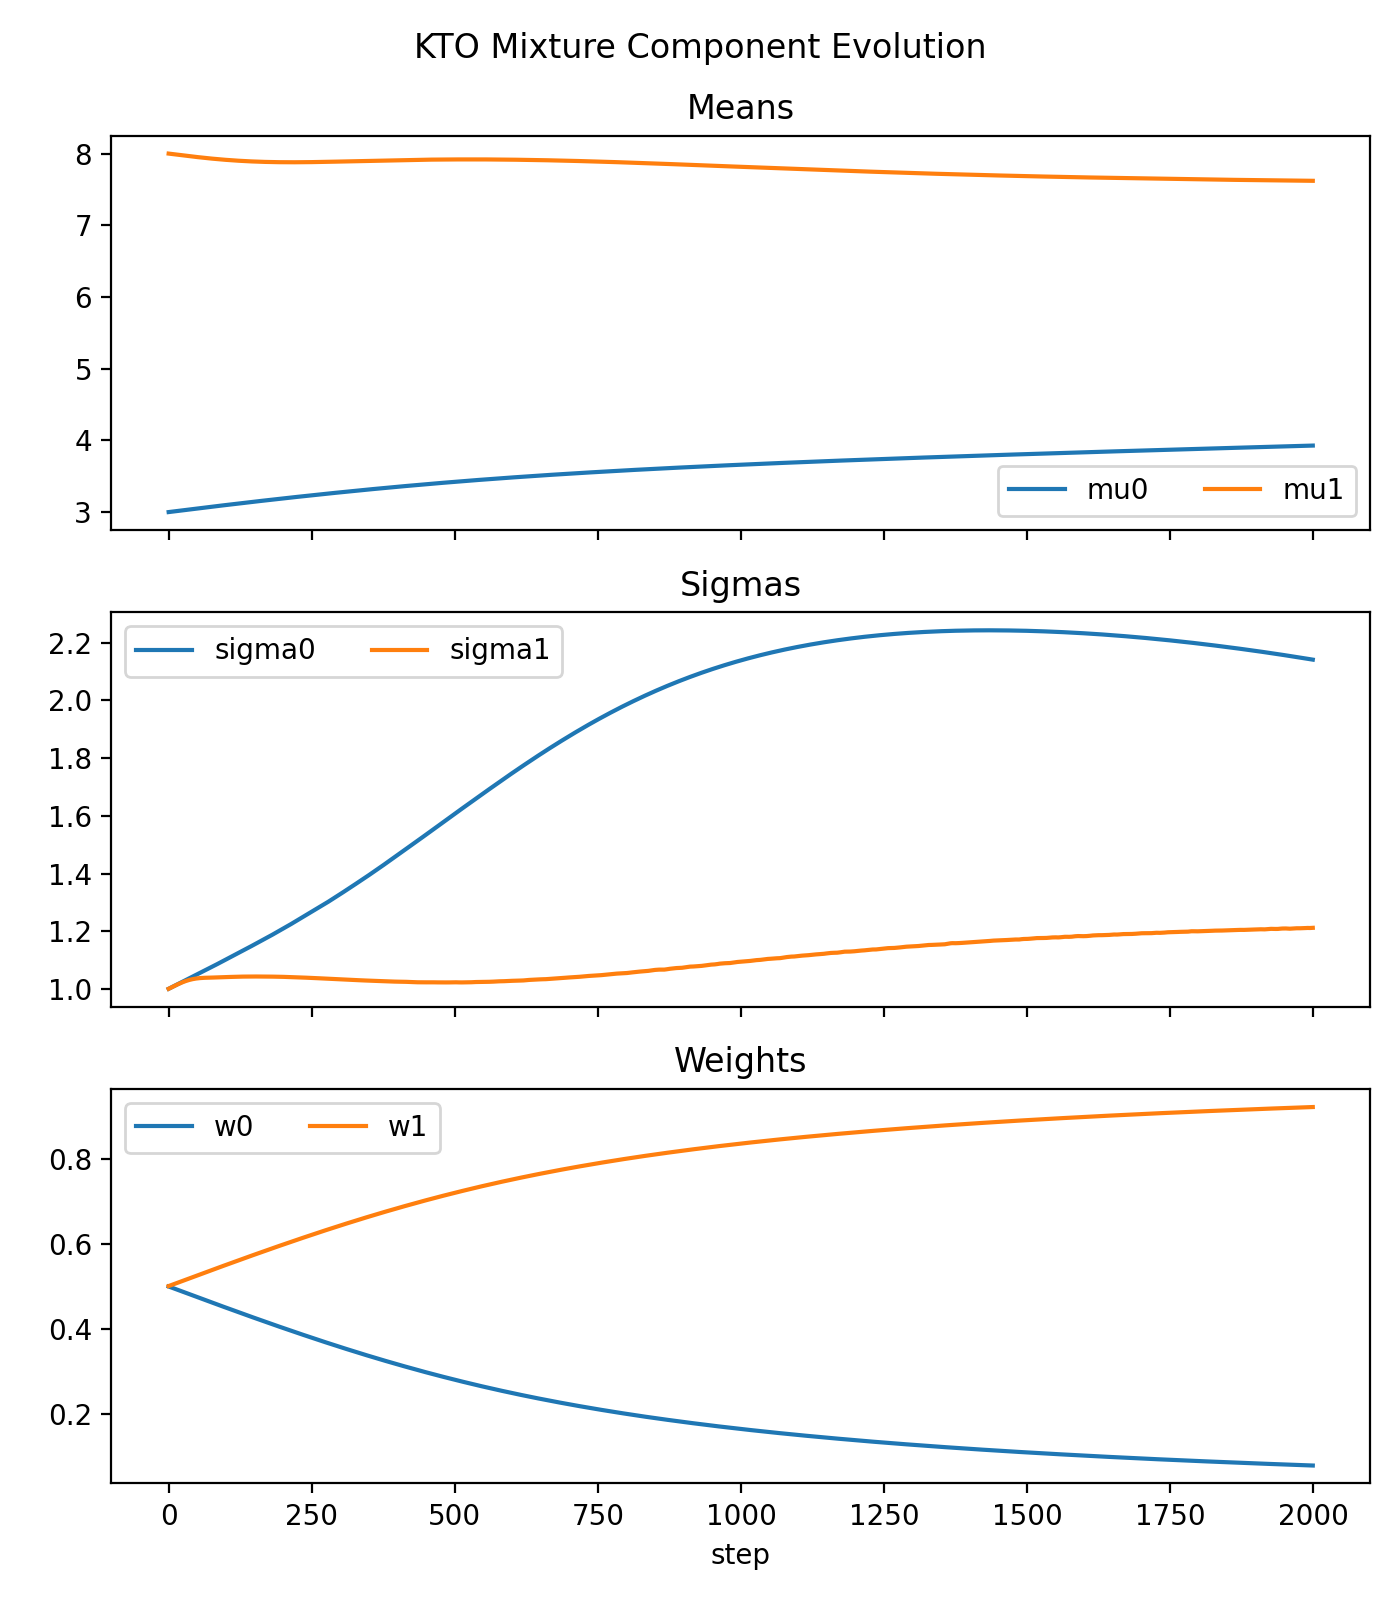
\includegraphics[width=0.95\textwidth]{figures/mix_component_evolution_kto.png}
    \caption{KTO mixture component evolution (mu, sigma, weights).}
\end{figure}

\begin{figure}[H]
    \centering
    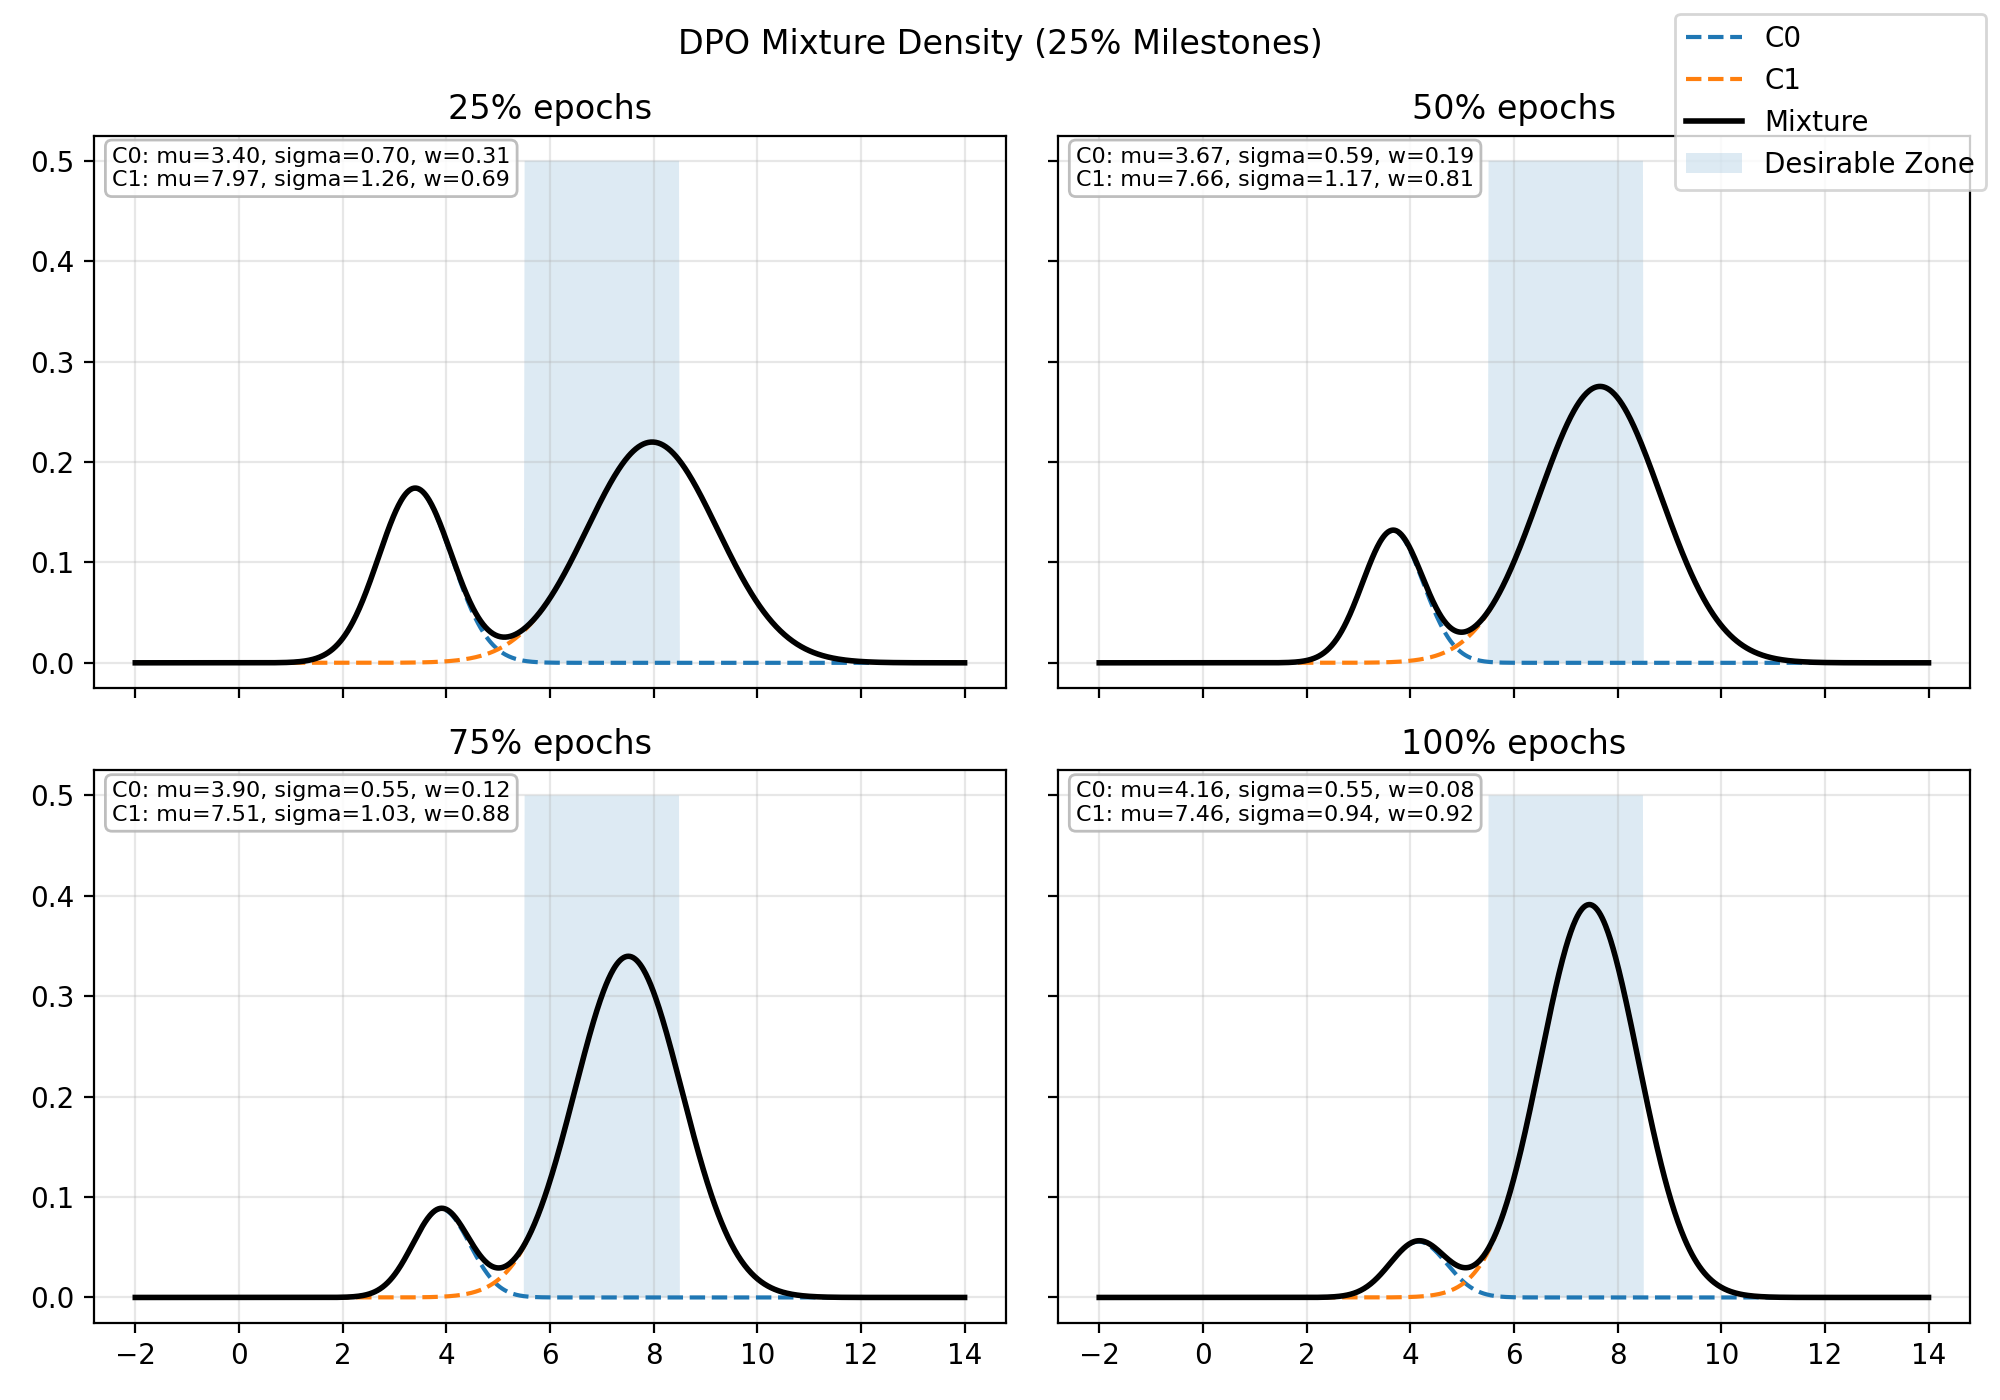
\includegraphics[width=0.95\textwidth]{figures/mix_density_milestones_dpo.png}
    \caption{DPO mixture density snapshots at 25\% milestones.}
\end{figure}

\begin{figure}[H]
    \centering
    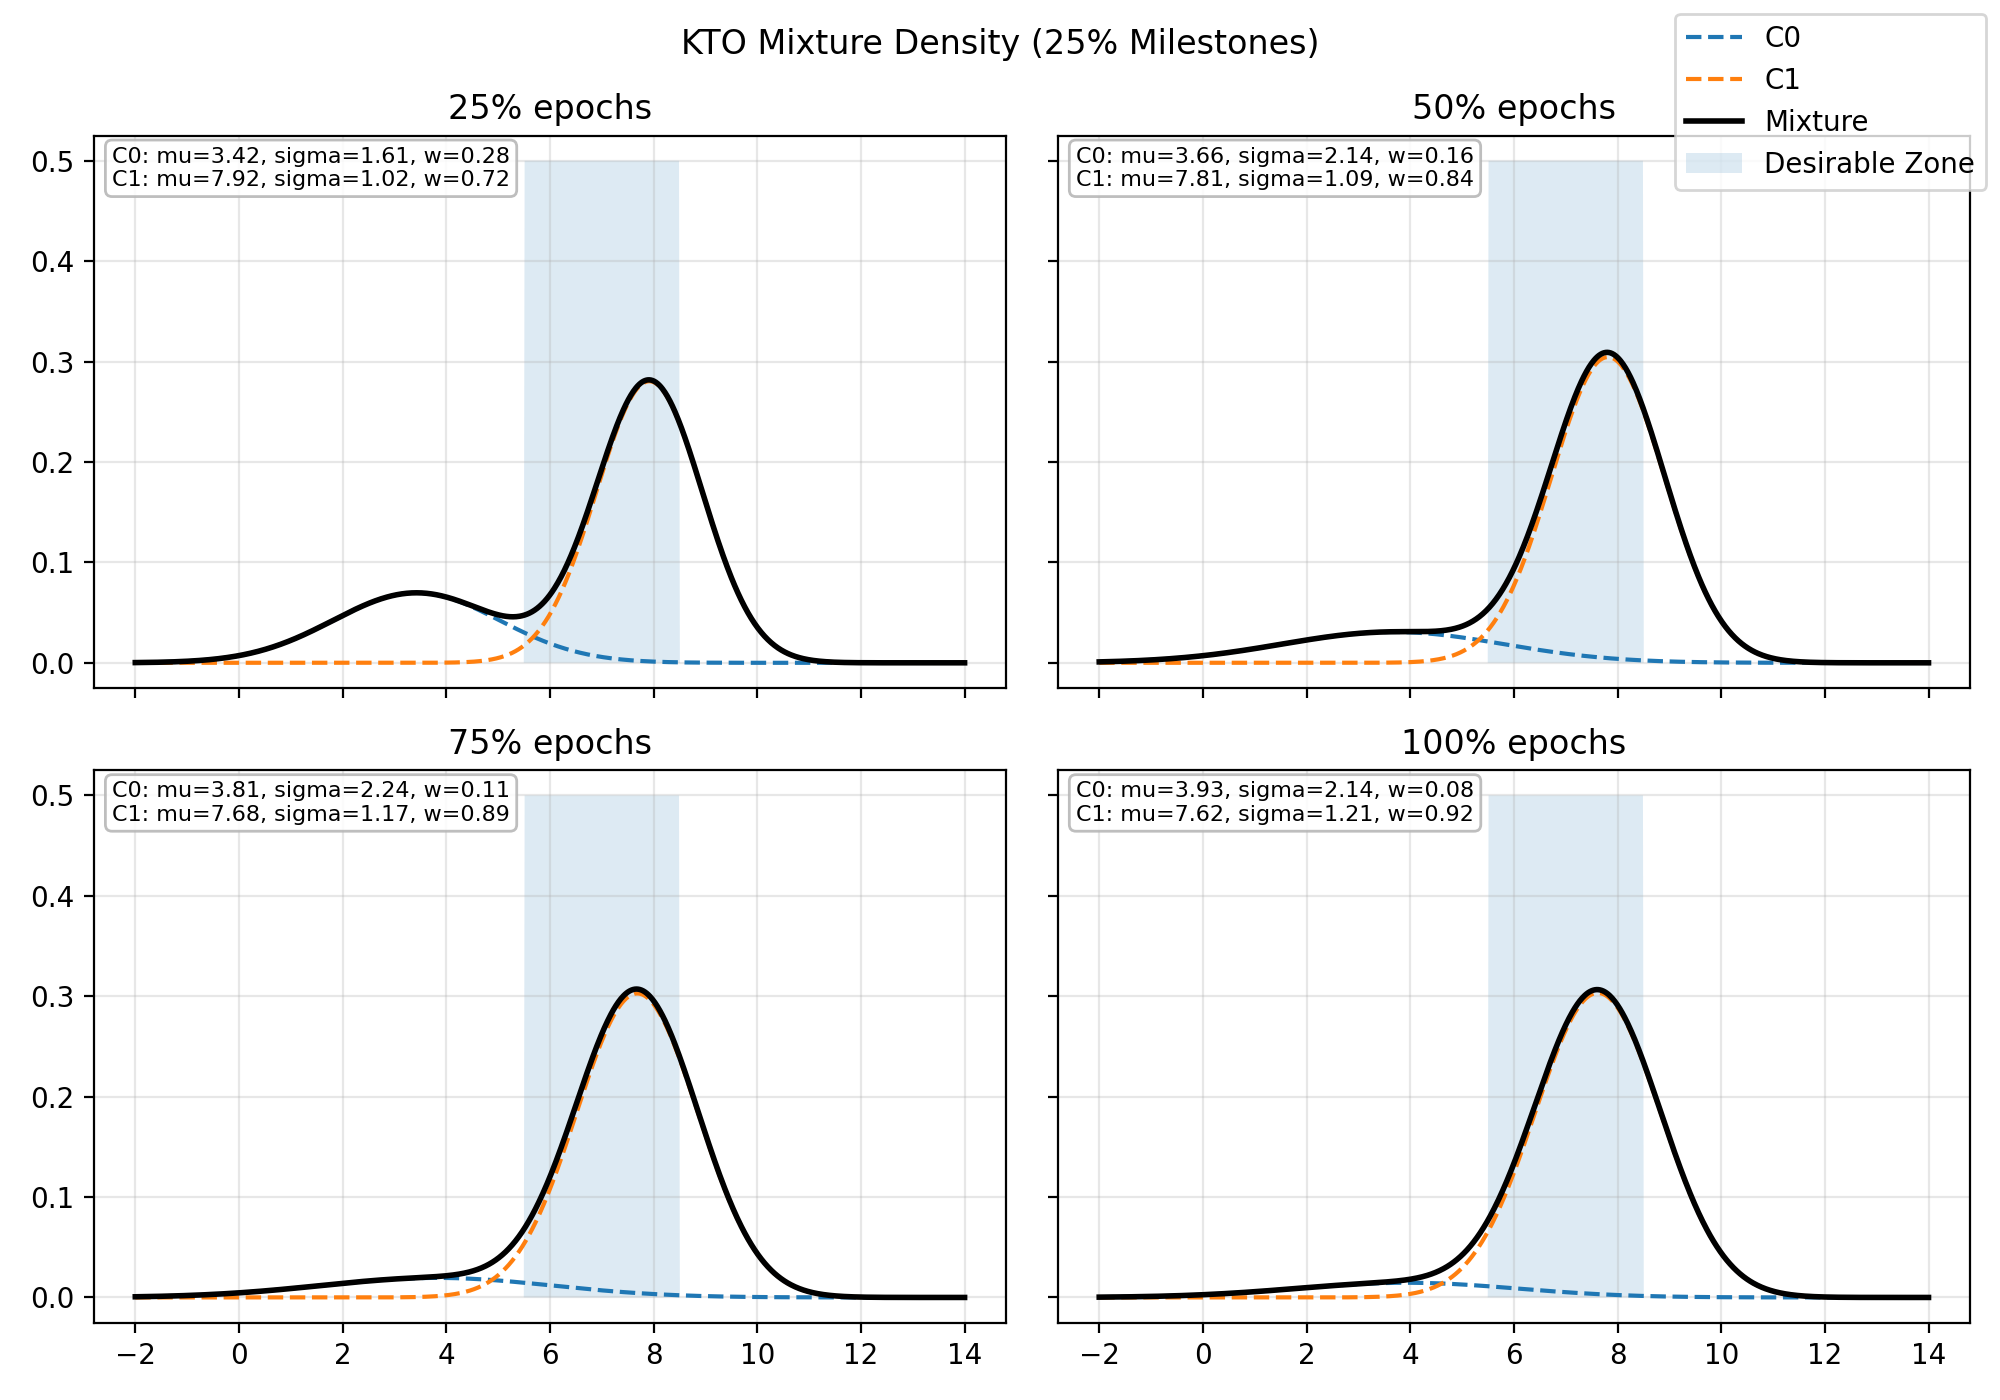
\includegraphics[width=0.95\textwidth]{figures/mix_density_milestones_kto.png}
    \caption{KTO mixture density snapshots at 25\% milestones.}
\end{figure}

\section{New: Robustness (Single vs Mixture)}
\begin{figure}[H]
    \centering
    
\includegraphics[width=0.95\textwidth]{figures/robustness_params_single_vs_mixture.png}
    \caption{Final parameters vs. data ratio (single vs mixture).}
\end{figure}

\begin{figure}[H]
    \centering
    
\includegraphics[width=0.95\textwidth]{figures/robustness_training_dynamics_single_vs_mixture.png}
    \caption{Training dynamics for the tracked DPO good\_ratio / KTO alpha setting (single vs mixture).}
\end{figure}

\section{Gaussian Mixture MLE (Auxiliary)}
\begin{figure}[H]
    \centering
    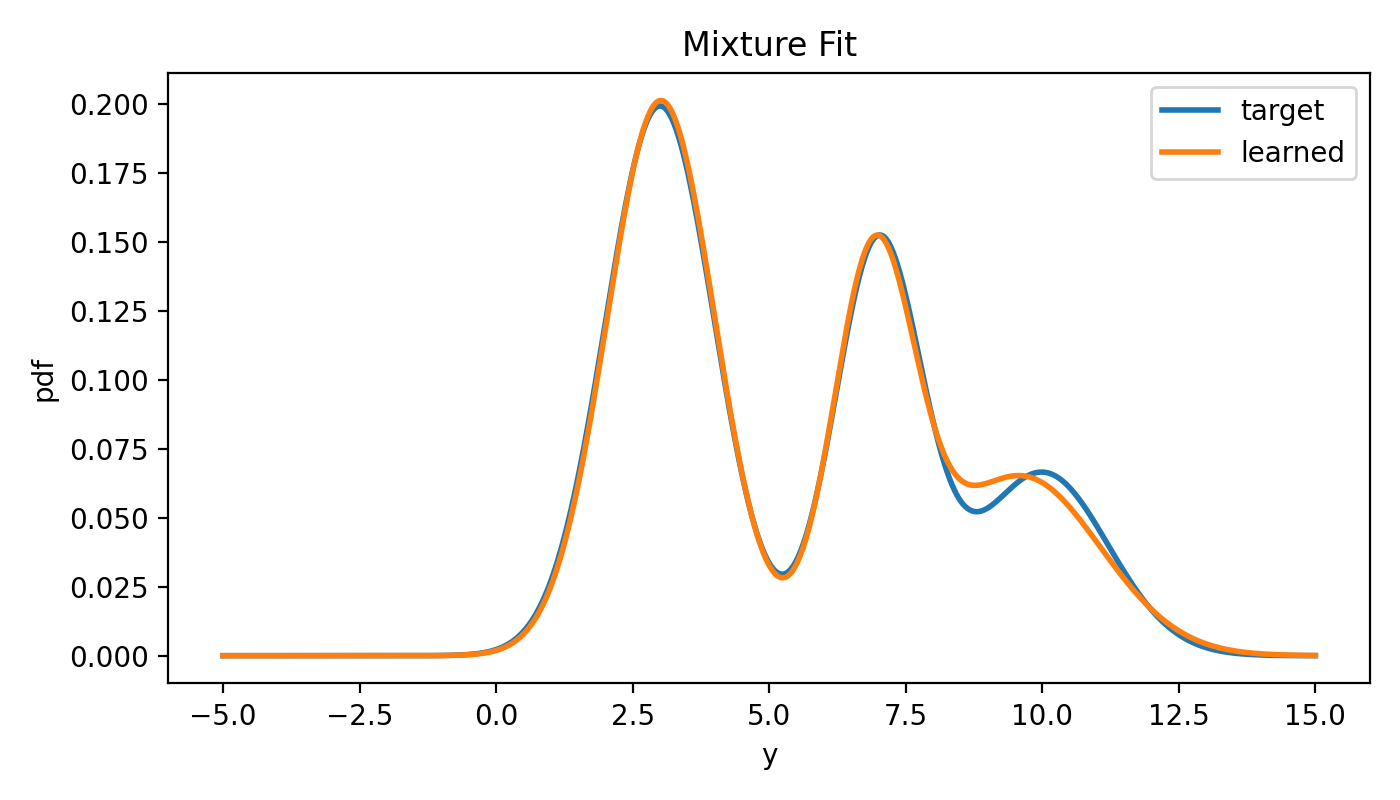
\includegraphics[width=0.85\textwidth]{figures/gaussian_mixture_fit.png}
    \caption{Target vs learned mixture density.}
\end{figure}

\begin{figure}[H]
    \centering
    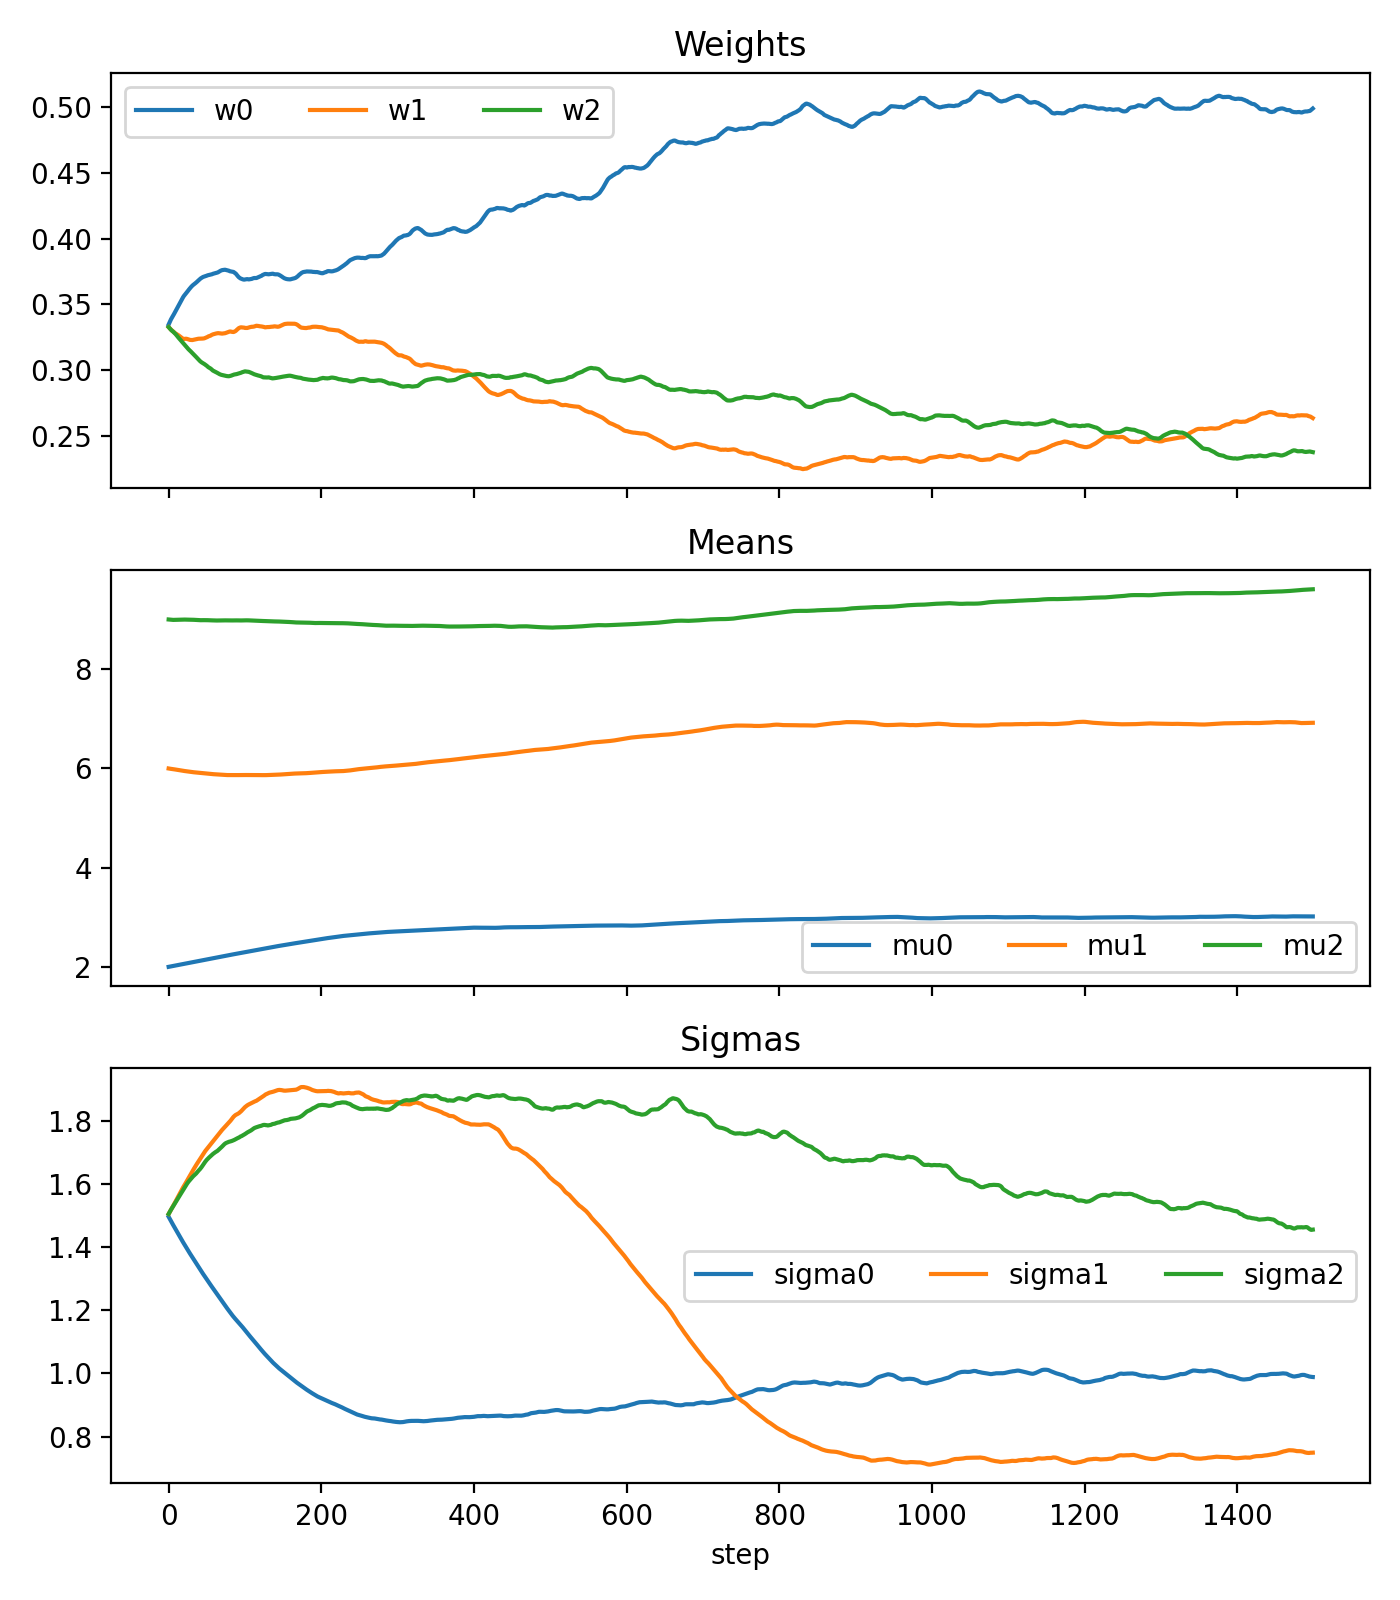
\includegraphics[width=0.85\textwidth]{figures/gaussian_mixture_evolution.png}
    \caption{Mixture parameter evolution (weights, means, sigmas).}
\end{figure}

\end{document}
